\section{Resultados Experimentales y Discusión Crítica}
\label{sec:resultados_experimentales_discusion}

En esta sección se presentan y discuten en profundidad los resultados empíricos obtenidos en las tres baterías de evaluación experimental diseñadas para contrastar las hipótesis $H_1$, $H_2$ y $H_3$. Se describe detalladamente la composición de los dos corpus audiovisuales de referencia y el catálogo de 138 consultas anotadas. A continuación, se expone el estudio de ablación dimensional guiado por \textit{Matryoshka Representation Learning} (MRL). Posteriormente, se evalúa el beneficio cuantitativo de la integración audio-visual y la verificación bimodal de segunda etapa frente a la línea base visual. Seguidamente, se analiza el comportamiento del sistema ante consultas multi-objetivo y consultas negativas de control para la discriminación de falsos positivos. Por último, se examina la eficiencia computacional, los desgloses de latencia granular y la escalabilidad de la huella de memoria vectorial, culminando con una comparativa empírica controlada entre el modelo propietario en la nube y dos codificadores locales abiertos (\textit{Qwen3-VL-Embedding-2B} y \textit{EmbeddingGemma 2}) ejecutados en Apple Silicon.

\subsection{Banco de Pruebas Experimental, Corpus Audiovisuales y Catálogo de Consultas}
\label{subsec:banco_pruebas_corpus}

Para evaluar rigurosamente las hipótesis de investigación $H_1$, $H_2$ y $H_3$, se diseñó un banco de pruebas empírico estructurado en torno a dos corpus de metraje continuo de vídeo con propiedades semánticas y de acoplamiento audiovisual diametralmente opuestas.

\subsubsection{Caracterización de los Corpus Audiovisuales de Referencia}
Los dos vídeos seleccionados totalizan $164$ fragmentos temporales indexados en la base vectorial local:
\begin{enumerate}
    \item \textbf{Dominio Técnico con Locución Sincronizada (\texttt{python\_tutorial.mp4}):} Metraje de $242,5\text{ s}$ de duración, correspondiente a una clase magistral de programación impartida por Brais Moure. Tras la segmentación adaptativa por SSIM en el banco E2E ($\theta_{\text{SSIM}} = 0,60, T_{\max} = 5,0\text{ s}$), se generan $82$ fragmentos temporales ($81/82$ con presencia de voz activa, $98,8\%$). En este dominio existe un acoplamiento temporal estricto entre lo que el ponente pronuncia verbalmente y las instrucciones sintácticas que se codifican en pantalla.
    \item \textbf{Dominio Documental con Metraje Desacoplado (\texttt{animals.mp4}):} Metraje de $243,0\text{ s}$ de duración perteneciente a un documental de naturaleza con locución en \textit{off} continua ($\theta_{\text{SSIM}} = 0,50, T_{\max} = 8,0\text{ s}$; $82$ fragmentos, $82/82$ con audio, $100,0\%$). Este metraje presenta el fenómeno clásico de \textit{B-roll desacoplado}: el narrador expone consideraciones taxonómicas y evolutivas generales mientras en pantalla se suceden planos de especies animales específicas que no son mencionadas textualmente en ese segundo concreto.
\end{enumerate}

\subsubsection{Taxonomía del Catálogo de Consultas Anotadas}
El banco de consultas comprende tres baterías de prueba disjuntas, diseñadas para someter al sistema a diferentes grados de dificultad perceptual y semántica:
\begin{itemize}
    \item \textbf{Batería 1: Consultas Literales de Evento Único (102 consultas):} Compuesta por $56$ consultas sobre \texttt{python\_tutorial.mp4} y $46$ consultas sobre \texttt{animals.mp4}. Cada consulta describe un instante o evento altamente específico (por ejemplo, \textit{``Símbolo de llaves tachado con cruz roja X''} o \textit{``León macho descansando tumbado''}), contando con un único intervalo temporal de verdad terreno (\textit{ground truth}).
    \item \textbf{Batería 2: Consultas Generales y Multi-Objetivo (20 consultas):} Evalúa la capacidad del sistema para recuperar categorías taxonómicas y patrones abstractos distribuidos en múltiples intervalos disjuntos del vídeo. Comprende $10$ consultas en \texttt{python\_tutorial.mp4} ($48$ intervalos válidos totales, tales como \textit{``Estructuras de datos (list, tuple, set, dict)''} o \textit{``Terminal mostrando salida de ejecución''}) y $10$ consultas en \texttt{animals.mp4} ($58$ intervalos válidos, tales como \textit{``Felinos''}, \textit{``Reptiles''}, \textit{``Aves''} o \textit{``Animales de color blanco y negro''}).
    \item \textbf{Batería 3: Consultas Negativas de Control (16 consultas):} Formada por $8$ consultas por vídeo referidas a conceptos formalmente ausentes del metraje (por ejemplo, \textit{``Definición de clases con class e \_\_init\_\_''} en Python, o \textit{``Tiburón blanco atacando en el océano''} en animales). Evalúa la inmunidad del sistema frente a alucinaciones y falsos positivos inducidos por similitud del coseno espuria en la Etapa 1.
\end{itemize}

\subsubsection{Métricas Formales de Evaluación}
El rendimiento del sistema se cuantifica mediante métricas estandarizadas en Recuperación de Información (\textit{Information Retrieval}):
\begin{itemize}
    \item \textbf{\textit{Recall@k} ($k \in \{1, 3, 5\}$):} Proporción de consultas literales donde el fragmento objetivo correcto se sitúa dentro de las primeras $k$ posiciones del ranking.
    \item \textbf{\textit{Mean Reciprocal Rank} (MRR):} Media del inverso del rango del primer resultado correcto:
    \begin{equation}
        \text{MRR} = \frac{1}{|Q|} \sum_{q=1}^{|Q|} \frac{1}{\text{rank}_q}
    \end{equation}
    \item \textbf{\textit{Interval Recall} y Precisión en Consultas Multi-Objetivo:} Proporción de intervalos temporales válidos recuperados respecto al total de intervalos esperados, y porcentaje de candidatos devueltos que son efectivamente pertinentes tras la evaluación del árbitro bimodal.
    \item \textbf{Tasa de Rechazo de Falsos Positivos:} Porcentaje de candidatos recuperados en consultas negativas que son correctamente identificados y descartados por el verificador de Etapa 2 con puntuación nula ($0,0$).
\end{itemize}

\newpage

\subsection{Estudio de Ablación Dimensional con Matryoshka Representation Learning (MRL)}
\label{subsec:ablacion_dimensional_mrl}

Para contrastar la Hipótesis 2 ($H_2$), se analizó el impacto del truncamiento prefijo y re-normalización $L_2$ sobre los $164$ fragmentos de los dos vídeos de referencia en las tres resoluciones dimensionales soportadas por \textit{Gemini Embedding 2}: $d = 3072$ (nativa), $d = 1536$ (reducción del $50\%$) y $d = 768$ (reducción del $75\%$).

\subsubsection{Fundamento Matemático del Truncado Prefijo y Re-Normalización $L_2$}
Cuando el codificador devuelve el vector nativo $\mathbf{v} \in \mathbb{R}^{3072}$, su norma euclídea es unitaria: $\|\mathbf{v}\|_2 = \sqrt{\sum_{j=1}^{3072} v_j^2} = 1,0$ \cite{gemini_emb2_docs}. Al truncar el vector a una sub-dimensión $d < 3072$ tomando sus primeras coordenadas $\mathbf{v}_{1:d} = (v_1, \dots, v_d)^\top$, se descartan las coordenadas de cola $[d+1 : 3072]$, por lo que la norma euclídea del sub-vector pasa a ser estrictamente inferior a la unidad:
\begin{equation}
    \|\mathbf{v}_{1:d}\|_2^2 = \sum_{j=1}^{d} v_j^2 = 1 - \sum_{j=d+1}^{3072} v_j^2 < 1,0
    \label{eq:perdida_norma_mrl}
\end{equation}

Si el sub-vector truncado se indexase en Qdrant sin corregir su magnitud, la métrica del coseno sobre grafos HNSW \cite{malkov2020hnsw} perdería invariancia geométrica porque el producto escalar dejaría de coincidir con el coseno del ángulo. Para restablecer la coherencia en todos los motores, \texttt{truncate\_and\_normalize\_mrl} en \texttt{src/embeddings/mrl.py} aplica un recorte prefijo seguido de re-normalización $L_2$ explícita:
\begin{equation}
    \hat{\mathbf{v}}_{1:d} = \frac{\mathbf{v}_{1:d}}{\|\mathbf{v}_{1:d}\|_2} = \frac{(v_1, v_2, \dots, v_d)^\top}{\sqrt{\sum_{j=1}^{d} v_j^2}}, \quad \text{con } \|\hat{\mathbf{v}}_{1:d}\|_2 = 1,0
    \label{eq:formula_mrl_l2_tex}
\end{equation}
En la arquitectura actual (\texttt{src/config.py}), las dimensiones admisibles por backend se declaran en \texttt{EMBEDDING\_\allowbreak BACKENDS} y cada pareja $(b, d)$ se aísla mediante \texttt{collection\_name\_for} junto con una clave \texttt{SHA-256} específica en caché para impedir colisiones entre resoluciones.

\subsubsection{Comportamiento en Consultas Literales de Evento Único}
El Cuadro~\ref{tab:ablacion_mrl_literales} sintetiza el rendimiento comparativo desglosado por corpus y agregado sobre el conjunto de las $102$ consultas literales en la Etapa 1 de recuperación densa en Qdrant, y la Figura~\ref{fig:grafica_compromiso_mrl} ilustra el compromiso entre precisión semántica, memoria y latencia.

\begin{table}[htbp]
\centering
\small
\setlength{\tabcolsep}{3.0pt}
\caption{Resultados de la ablación dimensional MRL sobre consultas literales de evento único ($102$ consultas, $164$ fragmentos en precisión \texttt{float32}) en la Etapa 1 (Qdrant).}
\label{tab:ablacion_mrl_literales}
\begin{adjustbox}{max width=\linewidth}
\begin{tabular}{llccccccc}
\toprule
\textbf{Corpus} & \textbf{Dim. ($d$)} & \textbf{\textit{Recall@1}} & \textbf{\textit{Recall@3}} & \textbf{\textit{Recall@5}} & \textbf{MRR} & \textbf{KB/vec} & \textbf{Ahorro} & \textbf{Latencia} \\
\midrule
\texttt{python\_tutorial} & $3072$ & $85,71\%$ ($48/56$) & $92,86\%$ ($52/56$) & $94,64\%$ ($53/56$) & $0,8973$ & $12,00$ & $0,0\%$ & $1,1688\text{ ms}$ \\
\texttt{python\_tutorial} & $1536$ & $85,71\%$ ($48/56$) & $92,86\%$ ($52/56$) & $96,43\%$ ($54/56$) & $0,9009$ & $6,00$ & $50,0\%$ & $0,7502\text{ ms}$ \\
\texttt{python\_tutorial} & $768$  & $85,71\%$ ($48/56$) & $92,86\%$ ($52/56$) & $\mathbf{98,21\%}$ ($55/56$) & $\mathbf{0,9045}$ & $3,00$ & $\mathbf{75,0\%}$ & $\mathbf{0,6297\text{ ms}}$ \\
\midrule
\texttt{animals.mp4}      & $3072$ & $\mathbf{71,74\%}$ ($33/46$) & $93,48\%$ ($43/46$) & $\mathbf{100,0\%}$ ($46/46$) & $\mathbf{0,8341}$ & $12,00$ & $0,0\%$ & $1,1104\text{ ms}$ \\
\texttt{animals.mp4}      & $1536$ & $69,57\%$ ($32/46$) & $93,48\%$ ($43/46$) & $\mathbf{100,0\%}$ ($46/46$) & $0,8232$ & $6,00$ & $50,0\%$ & $0,7848\text{ ms}$ \\
\texttt{animals.mp4}      & $768$  & $69,57\%$ ($32/46$) & $\mathbf{95,65\%}$ ($44/46$) & $\mathbf{100,0\%}$ ($46/46$) & $0,8261$ & $3,00$ & $\mathbf{75,0\%}$ & $\mathbf{0,6418\text{ ms}}$ \\
\midrule
\textbf{Global (102 q)}   & $3072$ & $\mathbf{79,41\%}$ ($81/102$) & $93,14\%$ ($95/102$) & $97,06\%$ ($99/102$) & $0,8688$ & $12,00$ & $0,0\%$ & $1,1425\text{ ms}$ \\
\textbf{Global (102 q)}   & $1536$ & $78,43\%$ ($80/102$) & $93,14\%$ ($95/102$) & $98,04\%$ ($100/102$) & $0,8659$ & $6,00$ & $50,0\%$ & $0,7658\text{ ms}$ \\
\textbf{Global (102 q)}   & $768$  & $78,43\%$ ($80/102$) & $\mathbf{94,12\%}$ ($96/102$) & $\mathbf{99,02\%}$ ($101/102$) & $\mathbf{0,8691}$ & $3,00$ & $\mathbf{75,0\%}$ & $\mathbf{0,6352\text{ ms}}$ \\
\bottomrule
\end{tabular}
\end{adjustbox}
\end{table}

\begin{figure}[htbp]
\centering
\begin{tikzpicture}
% Cuadrante 1: Métricas de Recuperación (Recall)
\begin{scope}
\draw[-stealth, thick, black!70] (0,0) -- (5.5,0);
\draw[-stealth, thick, black!70] (0,0) -- (0,3.95) node[above=2pt, font=\scriptsize\bfseries] {Porcentaje (\%)};

\foreach \y/\label in {0.6/75\%, 1.8/85\%, 3.0/95\%, 3.6/100\%} {
    \draw[gray!30, thin] (0,\y) -- (5.2,\y);
    \node[left=2pt, font=\tiny] at (0,\y) {\label};
}

\node[below=3pt, font=\scriptsize\bfseries] at (1.0,0) {$768$};
\node[below=3pt, font=\scriptsize\bfseries] at (2.7,0) {$1.536$};
\node[below=3pt, font=\scriptsize\bfseries] at (4.4,0) {$3.072$};
\node[below=16pt, font=\scriptsize\bfseries] at (2.7,0) {Dimensión ($d$)};

% Curva Recall@5 Global: 99.02% (3.48), 98.04% (3.36), 97.06% (3.25)
\draw[very thick, green!60!black] (1.0, 3.48) -- (2.7, 3.36) -- (4.4, 3.25);
\foreach \x/\y in {1.0/3.48, 2.7/3.36, 4.4/3.25} {
    \fill[green!60!black] (\x,\y) circle (2.2pt);
}
\node[above=3pt, font=\tiny\bfseries, green!55!black] at (1.0, 3.48) {R@5: 99,0\%};
\node[above=3pt, font=\tiny\bfseries, green!55!black] at (4.4, 3.25) {97,1\%};

% Curva Recall@3 Global: 94.12% (2.89), 93.14% (2.77), 93.14% (2.77)
\draw[thick, blue!80!black] (1.0, 2.89) -- (2.7, 2.77) -- (4.4, 2.77);
\foreach \x/\y in {1.0/2.89, 2.7/2.77, 4.4/2.77} {
    \node[fill=blue!80!black, minimum size=3.8pt, inner sep=0pt] at (\x,\y) {};
}
\node[below=3pt, font=\tiny\bfseries, blue!80!black] at (1.0, 2.89) {R@3: 94,1\%};
\node[below=3pt, font=\tiny\bfseries, blue!80!black] at (4.4, 2.77) {93,1\%};

% Curva Recall@1 Global: 78.43% (1.01), 78.43% (1.01), 79.41% (1.13)
\draw[very thick, red!80!black] (1.0, 1.01) -- (2.7, 1.01) -- (4.4, 1.13);
\foreach \x/\y in {1.0/1.01, 2.7/1.01, 4.4/1.13} {
    \node[regular polygon, regular polygon sides=3, fill=red!80!black, minimum size=4.8pt, inner sep=0pt] at (\x,\y) {};
}
\node[below=3pt, font=\tiny\bfseries, red!80!black] at (1.0, 1.01) {R@1: 78,4\%};
\node[above=3pt, font=\tiny\bfseries, red!80!black] at (4.4, 1.13) {79,4\%};

\node[font=\footnotesize\bfseries, align=center] at (2.7, 4.95) {(a) Precisión de Recuperación en Qdrant\\[-1pt]{\scriptsize\normalfont\textit{(Retención semántica $>98,8\%$ en R@1)}}};
\end{scope}

% Cuadrante 2: Eficiencia (Ahorro Memoria y Latencia)
\begin{scope}[xshift=7.8cm]
\draw[-stealth, thick, black!70] (0,0) -- (5.4,0);
\draw[-stealth, thick, blue!75!black] (0,0) -- (0,3.95) node[above=2pt, font=\scriptsize\bfseries, blue!75!black] {Ahorro RAM (\%)};
\draw[-stealth, thick, orange!80!black] (5.4,0) -- (5.4,3.95) node[above=2pt, font=\scriptsize\bfseries, orange!80!black] {Latencia (ms)};

\foreach \y/\label in {0.9/25\%, 1.8/50\%, 2.7/75\%, 3.6/100\%} {
    \draw[gray!30, thin] (0,\y) -- (5.4,\y);
    \node[left=2pt, font=\tiny, blue!75!black] at (0,\y) {\label};
}

\foreach \y/\label in {1.2/0{,}40, 2.4/0{,}80, 3.6/1{,}20} {
    \draw[orange!70!black, thin] (5.32,\y) -- (5.4,\y);
    \node[right=2pt, font=\tiny, orange!80!black] at (5.4,\y) {\label};
}

\node[below=3pt, font=\scriptsize\bfseries] at (1.0,0) {$768$};
\node[below=3pt, font=\scriptsize\bfseries] at (2.7,0) {$1.536$};
\node[below=3pt, font=\scriptsize\bfseries] at (4.4,0) {$3.072$};
\node[below=16pt, font=\scriptsize\bfseries] at (2.7,0) {Dimensión ($d$)};

\fill[blue!20, draw=blue!80!black] (0.42, 0) rectangle (1.58, 2.70);
\node[font=\tiny\bfseries, blue!90!black] at (1.0, 0.45) {+75\% RAM};

\fill[blue!20, draw=blue!80!black] (2.12, 0) rectangle (3.28, 1.80);
\node[font=\tiny\bfseries, blue!90!black] at (2.7, 0.45) {+50\% RAM};

\fill[blue!10, draw=blue!50!black] (3.82, 0) rectangle (4.98, 0.05);
\node[above=2pt, font=\tiny, text=gray!80!black] at (4.4, 0.08) {Línea base};

\draw[very thick, orange!85!black] (1.0, 1.91) -- (2.7, 2.30) -- (4.4, 3.43);
\foreach \x/\y in {1.0/1.91, 2.7/2.30, 4.4/3.43} {
    \node[diamond, fill=orange!85!black, minimum size=5pt, inner sep=0pt] at (\x,\y) {};
}
\node[below=4pt, font=\tiny\bfseries, orange!75!black] at (1.0, 1.91) {$0{,}64\text{ ms}$};
\node[above=4pt, font=\tiny\bfseries, orange!75!black, fill=white, inner sep=1pt] at (2.7, 2.30) {$0{,}77\text{ ms}$};
\node[left=4pt, font=\tiny\bfseries, orange!75!black, fill=white, inner sep=1pt] at (4.4, 3.43) {$1{,}14\text{ ms}$};

\node[font=\footnotesize\bfseries, align=center] at (2.7, 4.95) {(b) Eficiencia de Recursos\\[-1pt]{\scriptsize\normalfont\textit{(Ahorro de Almacenamiento y Latencia)}}};
\end{scope}
\end{tikzpicture}
\caption{Compromiso dimensional Matryoshka (MRL): (a) retención prácticamente plana de \textit{Recall@1} ($79,4\% \to 78,4\%$) con leve mejora en \textit{Recall@5} ($97,1\% \to 99,0\%$) frente a (b) reducción del $75\%$ en memoria RAM ($12\text{ KB} \to 3\text{ KB}$ por vector) y descenso del $44,4\%$ en la latencia de búsqueda en Qdrant.}
\label{fig:grafica_compromiso_mrl}
\end{figure}

El análisis desagregado consulta por consulta sobre los registros de auditoría revela patrones fundamentales sobre la estructura interna del subespacio Matryoshka:
\begin{enumerate}
    \item \textbf{Invarianza topológica en dominio con locución sincronizada (\texttt{python\_tutorial.mp4}):} En las $56$ consultas literales de Python, el \textit{Recall@1} se mantiene estrictamente invariante en un \textbf{$85,71\%$ ($48/56$)} y el \textit{Recall@3} en un \textbf{$92,86\%$ ($52/56$)} al pasar de $3072$ a $1536$ y $768$ dimensiones. La inspección individual confirma que $53$ de las $56$ consultas ($94,6\%$) conservan exactamente la misma posición en las tres resoluciones, sin pérdida alguna entre las $48$ consultas resueltas en primer puesto; de hecho, el \textit{MRR} asciende ligeramente de $0,8973$ ($d=3072$) a \textbf{$0,9045$ ($d=768$)}.
    \item \textbf{Efecto regularizador en \textit{Recall@5} sobre interfaces estáticas:} En $d=768$, el \textit{Recall@5} global aumenta del $97,06\%$ al \textbf{$99,02\%$ ($101/102$ consultas acertadas)}. Al transcurrir \texttt{python\_tutorial.mp4} sobre el fondo estático de Visual Studio Code, las coordenadas de cola ($[768:3072]$) capturan variaciones de alta frecuencia irrelevantes; al truncarlas, emergen dentro del \textit{Top-5} dos consultas que quedaban fuera en $3072\text{d}$: el símbolo de llaves tachado con cruz roja (que asciende al puesto \#5) y la salida de consola de \texttt{range(5)} (puesto \#4).
    \item \textbf{Estabilidad inter-dimensional y significación estadística en \texttt{animals.mp4} y agregado ($N=102$):} En el documental de naturaleza, $41$ de las $46$ consultas ($89,1\%$) conservan rango idéntico entre resoluciones (solo una consulta, la del ciervo con cornamenta, pasa del \#1 al \#2) y el \textit{Recall@5} permanece en el $100,0\%$ ($46/46$). En las pruebas pareadas globales ($3072\text{d} \to 768\text{d}$, $N=102$), las diferencias resultan estadísticamente indistinguibles tanto en \textit{Recall@1} (prueba exacta de \textit{McNemar} $p = 1,0000$) como en \textit{MRR} (prueba de \textit{Wilcoxon} $p = 0,6729$), confirmando que la compresión MRL preserva íntegramente la distribución de rangos.
\end{enumerate}

\subsubsection{Validación Cuantitativa de la Hipótesis 2 ($H_2$)}
Los resultados confirman con holgura la Hipótesis 2: la compresión del espacio latente a $d = 768$ dimensiones (reducción del $75\%$ en huella de memoria) retiene el \textbf{$98,77\%$ del \textit{Recall@1} relativo}, preserva un \textit{MRR} equivalente ($0,8691$ vs. $0,8688$; $p = 0,6729$) y reduce la latencia de cómputo en Qdrant en un \textbf{$44,4\%$}, permitiendo escalar la capacidad vectorial por un factor de $4\times$ sin merma apreciable.

\newpage

\subsection{Evaluación Empírica de la Integración Audio-Visual y Verificación Bimodal}
\label{subsec:evaluacion_audio_visual_e2e}

Esta subsección aborda directamente la Pregunta de Investigación 1 (\textbf{RQ1}) y la Hipótesis 1 ($H_1$), evaluando el beneficio de la fusión temprana de la pista de voz alineada frente a la línea base puramente visual, así como el papel corrector del juez bimodal de segunda etapa.

\subsubsection{Comparativa de Rendimiento: Línea Base Visual frente a Fusión Bimodal}
El Cuadro~\ref{tab:ablacion_visual_vs_audio_consolidado} expone las métricas comparativas entre la arquitectura puramente visual (3 fotogramas clave por plano) y la arquitectura bimodal completa (3 fotogramas + transcripción Whisper alineada + verificación bimodal con \textit{Gemini 3.5 Flash Lite}) en los dos dominios audiovisuales evaluados.

\begin{table}[htbp]
\centering
\small
\setlength{\tabcolsep}{4.0pt}
\caption{Comparativa empírica entre la arquitectura puramente visual y la canalización bimodal con fusión temprana de audio y verificación en dos etapas.}
\label{tab:ablacion_visual_vs_audio_consolidado}
\begin{tabular}{lllccc}
\toprule
\textbf{Corpus de Vídeo} & \textbf{Etapa del Sistema} & \textbf{Métrica de IR} & \textbf{Línea Base Visual} & \textbf{Fusión Bimodal} & \textbf{Variación} \\
\midrule
\texttt{python\_tutorial.mp4} & Etapa 1 (Qdrant) & \textit{Recall@1} & $67,9\%$ ($38/56$) & $\mathbf{85,7\%}$ ($48/56$) & $\mathbf{+17,8\text{ pp}}$ \\
\texttt{python\_tutorial.mp4} & Etapa 1 (Qdrant) & \textit{Recall@3} & $87,5\%$ ($49/56$) & $\mathbf{92,9\%}$ ($52/56$) & $\mathbf{+5,4\text{ pp}}$ \\
\texttt{python\_tutorial.mp4} & Etapa 1 (Qdrant) & \textit{MRR} & $0,779$ & $\mathbf{0,897}$ & $\mathbf{+0,118}$ \\ \addlinespace[2.5pt]
\texttt{python\_tutorial.mp4} & Etapa 2 (Juez Bimodal) & \textit{Recall@1} & $80,4\%$ ($45/56$) & $\mathbf{89,3\%}$ ($50/56$) & $\mathbf{+8,9\text{ pp}}$ \\
\texttt{python\_tutorial.mp4} & Etapa 2 (Juez Bimodal) & \textit{MRR} & $0,848$ & $\mathbf{0,911}$ & $\mathbf{+0,063}$ \\
\midrule
\texttt{animals.mp4} & Etapa 1 (Qdrant) & \textit{Recall@1} & $\mathbf{80,4\%}$ ($37/46$) & $71,7\%$ ($33/46$) & $-8,7\text{ pp}$ \\
\texttt{animals.mp4} & Etapa 1 (Qdrant) & \textit{Recall@5} & $95,7\%$ ($44/46$) & $\mathbf{100,0\%}$ ($46/46$) & $\mathbf{+4,3\text{ pp}}$ \\ \addlinespace[2.5pt]
\texttt{animals.mp4} & Etapa 2 (Juez Bimodal) & \textit{Recall@1} & $89,1\%$ ($41/46$) & $\mathbf{93,5\%}$ ($43/46$) & $\mathbf{+4,4\text{ pp}}$ \\
\texttt{animals.mp4} & Etapa 2 (Juez Bimodal) & \textit{Recall@5} & $93,5\%$ ($43/46$) & $\mathbf{97,8\%}$ ($45/46$) & $\mathbf{+4,3\text{ pp}}$ \\
\texttt{animals.mp4} & Etapa 2 (Juez Bimodal) & \textit{MRR} & $0,913$ & $\mathbf{0,951}$ & $\mathbf{+0,038}$ \\
\bottomrule
\end{tabular}
\end{table}

\subsubsection{Discusión de Fenómenos Perceptuales}
Los datos empíricos revelan dos dinámicas fundamentales:
\begin{enumerate}
    \item \textbf{Convergencia Modal en Metraje Educativo:} En \texttt{python\_tutorial.mp4}, la inyección de la locución hablada produce una ganancia masiva de $+17,8$ puntos porcentuales en \textit{Recall@1} en la primera etapa ($67,9\% \to 85,7\%$). La coincidencia temporal entre el código tecleado y la explicación oral del ponente refuerza la densidad direccional del embedding omnimodal, posicionando 10 consultas adicionales directamente en el primer lugar del ranking sin requerir reordenación. Tras la actuación del verificador en la Etapa 2, el \textit{Recall@1} alcanza el **$89,3\%$ ($50/56$)** con un \textit{MRR} de **$0,911$**.
    \item \textbf{Compensación Asimétrica ante Metraje Desacoplado (\textit{B-roll}):} En \texttt{animals.mp4}, donde la narración verbal describe conceptos biológicos mientras la cámara enfoca especies que no son mencionadas por su nombre, la fusión de audio induce una leve desviación en la primera etapa ($\Delta\text{\textit{Recall@1}} = -8,7\text{ pp}$). Sin embargo, la cobertura en \textit{Recall@5} asciende al **$100,0\%$ ($46/46$)**, garantizando que el fragmento correcto jamás es descartado por el motor vectorial. Posteriormente, el árbitro bimodal de Etapa 2 analiza de forma disjunta la evidencia visual y auditiva, corrigiendo por completo el desfase y alcanzando un récord de **$93,5\%$ de \textit{Recall@1}** ($43/46$) y un **$97,8\%$ de \textit{Recall@5}** con un \textit{MRR} de **$0,951$**.
\end{enumerate}

\subsubsection{Validación Cuantitativa de la Hipótesis 1 ($H_1$)}
Se confirma plenamente la Hipótesis 1: la fusión temprana audio-visual incrementa sustancialmente la precisión en contenidos sincronizados (+17,8 pp en \textit{Recall@1}) y, combinada con la verificación bimodal de segunda etapa, neutraliza el desacoplamiento en secuencias de tipo \textit{B-roll}, superando a la línea base visual en ambos dominios audiovisuales.

\newpage

\subsection{Evaluación en Consultas Complejas: Multi-Objetivo y Control Negativo}
\label{subsec:consultas_complejas}

Esta subsección contrasta la Hipótesis 3 ($H_3$) y la Pregunta de Investigación 3 (\textbf{RQ3}), analizando el comportamiento de la arquitectura en dos etapas ante consultas multi-intervalo y consultas con conceptos ausentes.

\subsubsection{Consultas Generales y Multi-Objetivo (Batería 2)}
Las consultas multi-objetivo evalúan la capacidad del sistema para recuperar conceptos de alto nivel semántico distribuidos a lo largo del metraje. El Cuadro~\ref{tab:multi_target_resumen} sintetiza los resultados para las 20 consultas generales ($106$ intervalos esperados en total) evaluadas con $k_1 = 10$.

\begin{table}[htbp]
\centering
\small
\setlength{\tabcolsep}{3.5pt}
\caption{Rendimiento en consultas multi-objetivo ($20$ consultas, $106$ intervalos esperados, $k_1 = 10$) en Etapa 1 (Qdrant) y Etapa 2 (Juez Bimodal).}
\label{tab:multi_target_resumen}
\begin{adjustbox}{max width=\linewidth}
\begin{tabular}{lccccccc}
\toprule
\textbf{Corpus de Vídeo} & \begin{tabular}[c]{@{}c@{}}\textbf{Dimensión}\\\textbf{($d$)}\end{tabular} & \textbf{Intervalos} & \begin{tabular}[c]{@{}c@{}}\textbf{Recall}\\\textbf{Etapa 1}\end{tabular} & \begin{tabular}[c]{@{}c@{}}\textbf{Precisión}\\\textbf{Etapa 1}\end{tabular} & \begin{tabular}[c]{@{}c@{}}\textbf{Recall}\\\textbf{Etapa 2}\end{tabular} & \begin{tabular}[c]{@{}c@{}}\textbf{Precisión}\\\textbf{Etapa 2}\end{tabular} & \begin{tabular}[c]{@{}c@{}}\textbf{\textit{Hit@1}}\\\textbf{Etapa 2}\end{tabular} \\
\midrule
\texttt{python\_tutorial.mp4} & $d = 3072$ & 48 & $85,42\%$ ($40/48$) & $45,00\%$ & $82,08\%$ ($38/48$) & $78,65\%$ & $9/10$ ($90,0\%$) \\
\texttt{python\_tutorial.mp4} & $d = 1536$ & 48 & $87,08\%$ ($41/48$) & $\mathbf{47,00\%}$ & $82,08\%$ ($38/48$) & $78,12\%$ & $9/10$ ($90,0\%$) \\
\texttt{python\_tutorial.mp4} & $d = 768$  & 48 & $\mathbf{87,22\%}$ ($41/48$) & $46,00\%$ & $\mathbf{83,89\%}$ ($40/48$) & $\mathbf{80,06\%}$ & $9/10$ ($90,0\%$) \\
\midrule
\texttt{animals.mp4} & $d = 3072$ & 58 & $\mathbf{74,89\%}$ ($42/58$) & $\mathbf{50,00\%}$ & $\mathbf{71,64\%}$ ($40/58$) & $\mathbf{96,57\%}$ & $\mathbf{10/10}$ ($\mathbf{100,0\%}$) \\
\texttt{animals.mp4} & $d = 1536$ & 58 & $71,98\%$ ($40/58$) & $48,00\%$ & $68,73\%$ ($38/58$) & $96,33\%$ & $\mathbf{10/10}$ ($\mathbf{100,0\%}$) \\
\texttt{animals.mp4} & $d = 768$  & 58 & $\mathbf{74,89\%}$ ($42/58$) & $\mathbf{50,00\%}$ & $\mathbf{71,64\%}$ ($40/58$) & $\mathbf{96,57\%}$ & $\mathbf{10/10}$ ($\mathbf{100,0\%}$) \\
\bottomrule
\end{tabular}
\end{adjustbox}
\end{table}

El Cuadro~\ref{tab:desglose_taxonomico_animals} desglosa por categoría cada una de las $10$ consultas generales sobre \texttt{animals.mp4}, ilustrando cómo la precisión media se duplica al pasar del \textbf{$50,00\%$ en Etapa 1 al $96,57\%$ en Etapa 2} y cómo el árbitro bimodal garantiza un \textit{Hit@1} del \textbf{$100,0\%$ ($10/10$)} en las tres dimensiones.

\begin{table}[htbp]
\centering
\small
\setlength{\tabcolsep}{4.0pt}
\caption{Desglose por consulta general y taxonómica sobre \texttt{animals.mp4} ($10$ consultas, $58$ intervalos temporales esperados) en Etapa 1 (E1) y Etapa 2 (E2).}
\label{tab:desglose_taxonomico_animals}
\begin{tabularx}{\linewidth}{>{\raggedright\arraybackslash}X c *{3}{>{\centering\arraybackslash}p{0.82cm}} *{3}{>{\centering\arraybackslash}p{0.88cm}} c}
\toprule
\multirow{2}{*}{\textbf{Consulta General / Taxonómica}} & \multirow{2}{*}{\textbf{Obj.}} & \multicolumn{3}{c}{\textbf{Etapa 1 (Qdrant)}} & \multicolumn{3}{c}{\textbf{Etapa 2 (Verificador)}} & \multirow{2}{*}{\textbf{Prec. E2}} \\
\cmidrule(lr){3-5} \cmidrule(lr){6-8}
& & \textbf{$3072$} & \textbf{$1536$} & \textbf{$768$} & \textbf{$3072$} & \textbf{$1536$} & \textbf{$768$} & \\
\midrule
\texttt{Felinos} & $4$ & $1/4$ & $1/4$ & $1/4$ & $1/4$ & $1/4$ & $1/4$ & $100,0\%$ \\
\texttt{Reptiles} & $2$ & $2/2$ & $2/2$ & $2/2$ & $2/2$ & $2/2$ & $2/2$ & $100,0\%$ \\
\texttt{Aves} & $4$ & $2/4$ & $2/4$ & $2/4$ & $2/4$ & $2/4$ & $2/4$ & $100,0\%$ \\
\texttt{Manada o grupo $\ge 3$ animales} & $10$ & $4/10$ & $4/10$ & $4/10$ & $4/10$ & $4/10$ & $4/10$ & $100,0\%$ \\
\texttt{Animales color blanco y negro} & $5$ & $5/5$ & $5/5$ & $5/5$ & $4/5$ & $4/5$ & $4/5$ & $100,0\%$ \\
\texttt{Animales marinos / acuáticos} & $8$ & $6/8$ & $5/8$ & $6/8$ & $6/8$ & $5/8$ & $6/8$ & $100,0\%$ \\
\texttt{Animales comiendo o pastando} & $8$ & $7/8$ & $7/8$ & $7/8$ & $6/8$ & $6/8$ & $6/8$ & $100,0\%$ \\
\texttt{Crías o animales jóvenes} & $7$ & $5/7$ & $5/7$ & $5/7$ & $5/7$ & $5/7$ & $5/7$ & $80,0\%$ \\
\texttt{Primer plano macro de ojos/orejas} & $6$ & $6/6$ & $5/6$ & $6/6$ & $6/6$ & $5/6$ & $6/6$ & $85,7\%$ \\
\texttt{Animación 3D microscópica células} & $4$ & $4/4$ & $4/4$ & $4/4$ & $4/4$ & $4/4$ & $4/4$ & $100,0\%$ \\
\bottomrule
\end{tabularx}
\end{table}

El examen individual de ambas baterías revela tres propiedades clave: (1) en \texttt{animals.mp4}, $d=768$ obtiene \textbf{exactamente los mismos aciertos por categoría} que $d=3072$ con idéntica precisión media ($96,57\%$); (2) cuando la voz en \textit{off} desplaza el primer acierto en Qdrant (como \textit{``Reptiles''}, en puesto \#4 en $3072$, \#2 en $1536$ y \#5 en $768$), el árbitro bimodal reordena la ventana $K=10$ y sitúa un acierto verdadero en el puesto \#1 en el $100,0\%$ de los casos ($10/10$); y (3) en \texttt{python\_tutorial.mp4}, $d=768$ eleva la cobertura sobre estructuras de datos (\texttt{list}, \texttt{tuple}, \texttt{set}, \texttt{dict}) del $5/6$ al $100,0\%$ ($6/6$) y los rótulos sobreimpresos de $3/8$ a $4/8$.

\subsubsection{Consultas Negativas de Control e Inmunidad a Falsos Positivos (Batería 3)}
Las búsquedas aproximadas basadas en similitud del coseno devuelven obligatoriamente los $k$ candidatos con mayor producto escalar, con independencia de que el concepto consultado exista o no en el corpus.

Para evaluar la capacidad de discriminación del sistema, se ejecutaron $16$ consultas negativas de control ($8$ sobre \texttt{python\_tutorial.mp4} y $8$ sobre \texttt{animals.mp4}) a través de las tres dimensiones MRL ($48$ ejecuciones y $240$ evaluaciones de candidatos con \textit{Gemini 3.5 Flash Lite}), cuyos resultados figuran en el Cuadro~\ref{tab:ablacion_mrl_negativas}:
\begin{itemize}
    \item \textbf{Etapa 1 (Qdrant sin umbral):} Devuelve $240/240$ candidatos ($100\%$ de falsos positivos potenciales), dado que los fragmentos de mayor similitud superficial corresponden a planos visualmente parecidos pero temáticamente erróneos.
    \item \textbf{Etapa 2 (Árbitro Bimodal):} Descarta el \textbf{$100,0\%$ de los candidatos} ($0/240$ falsos positivos admitidos), asignando a cada fragmento una puntuación de $0,0$ con la justificación explícita de ausencia de evidencia visual y auditiva.
\end{itemize}

\begin{table}[htbp]
\centering
\small
\setlength{\tabcolsep}{4.0pt}
\caption{Evaluación de consultas negativas de control ($16$ consultas, $240$ candidatos analizados en Etapa 2) a través de las tres dimensiones MRL.}
\label{tab:ablacion_mrl_negativas}
\begin{tabular}{llcccc}
\toprule
\textbf{Corpus de Vídeo} & \textbf{Dim. ($d$)} & \textbf{Consultas} & \textbf{Candidatos E1} & \textbf{Falsos Pos. E2} & \textbf{Tasa Rechazo E2} \\
\midrule
\texttt{python\_tutorial.mp4} & $3072$ & $8$ & $40$ & $\mathbf{0/40}$ ($0,0\%$) & $\mathbf{100,0\%}$ ($8/8$) \\
\texttt{python\_tutorial.mp4} & $1536$ & $8$ & $40$ & $\mathbf{0/40}$ ($0,0\%$) & $\mathbf{100,0\%}$ ($8/8$) \\
\texttt{python\_tutorial.mp4} & $768$  & $8$ & $40$ & $\mathbf{0/40}$ ($0,0\%$) & $\mathbf{100,0\%}$ ($8/8$) \\
\midrule
\texttt{animals.mp4}          & $3072$ & $8$ & $40$ & $\mathbf{0/40}$ ($0,0\%$) & $\mathbf{100,0\%}$ ($8/8$) \\
\texttt{animals.mp4}          & $1536$ & $8$ & $40$ & $\mathbf{0/40}$ ($0,0\%$) & $\mathbf{100,0\%}$ ($8/8$) \\
\texttt{animals.mp4}          & $768$  & $8$ & $40$ & $\mathbf{0/40}$ ($0,0\%$) & $\mathbf{100,0\%}$ ($8/8$) \\
\midrule
\textbf{Total Global (3 dim.)} & \textbf{Todas} & $\mathbf{48\text{ ejec.}}$ & $\mathbf{240}$ & $\mathbf{0/240}$ ($\mathbf{0,0\%}$) & $\mathbf{100,0\%}$ ($\mathbf{48/48}$) \\
\bottomrule
\end{tabular}
\end{table}

Este resultado confirma que el truncamiento dimensional ($3072 \to 1536 \to 768$) no induce colapso semántico ni degrada la especificidad del verificador bimodal.

\subsubsection{Validación Cuantitativa de la Hipótesis 3 ($H_3$)}
La Hipótesis 3 queda confirmada empíricamente: la verificación bimodal con un modelo de lenguaje multimodal erradica por completo los falsos positivos derivados de la similitud del coseno (tasa de rechazo del $100,0\%$) y eleva la precisión en consultas generales complejas por encima del $96\%$.

\newpage

\subsection{Análisis de Eficiencia Computacional, Latencias y Huella de Almacenamiento}
\label{subsec:eficiencia_computacional_costes}

Esta subsección analiza la viabilidad computacional y operativa de la arquitectura propuesta, evaluando los desgloses de latencia por etapa, la escalabilidad de almacenamiento vectorial y los compromisos de diseño para su adopción en entornos de producción.

\subsubsection{Desglose Granular de Latencias}
El arnés de auditoría \texttt{RunAuditor} registró los tiempos de ejecución de cada componente del prototipo:
\begin{itemize}
    \item \textbf{Segmentación Visual (SSIM):} La optimización sobre miniaturas de 160 px alcanza un rendimiento de procesamiento de aproximadamente $45\text{ FPS}$ en CPU Apple Silicon, procesando un vídeo de 4 minutos en menos de $6\text{ segundos}$.
    \item \textbf{Transcripción Whisper Local:} El modelo \texttt{base} transcribe y alinea temporalmente los 4 minutos de audio en aproximadamente $12\text{ segundos}$ en CPU local, operando en paralelo con la segmentación visual.
    \item \textbf{Vectorización en Gemini API frente a Inferencia Local (Etapa 1):} La llamada remota para vectorizar fragmentos con \textit{Gemini Embedding 2} presenta una mediana por consulta de $464\text{--}481\text{ ms}$ (unos $650\text{ ms}$ de media en invocación aislada multimodal y $187\text{--}227\text{ s}$ totales para indexar $82$ fragmentos bajo control de reintentos), mientras que la ejecución local en \texttt{bfloat16} sobre Metal MPS reduce la mediana de consulta a $91\text{--}98\text{ ms}$ en \texttt{qwen3-vl-2b} ($126\text{--}142\text{ s}$ de indexación) y a $\sim 30\text{ ms}$ en \texttt{gemma2} ($2,55\text{--}2,59\text{ GB}$ de memoria Metal), tal como se profundiza en la Subsección~\ref{subsec:comparativa_backends_locales}.
    \item \textbf{Búsqueda Vectorial en Qdrant (Etapa 1):} La consulta sobre el grafo HNSW se completa en $1,14\text{ ms}$ para $d=3072$ y se reduce a \textbf{$0,63\text{ ms}$ para $d=768$} (aceleración del $44,4\%$).
    \item \textbf{Verificación con Árbitro Bimodal (Etapa 2):} La llamada concurrente asíncrona a \textit{Gemini 3.5 Flash Lite} para evaluar y clasificar los 5 mejores candidatos requiere una latencia media de $1,4\text{ s}$, compatible con interfaces de usuario interactivas.
\end{itemize}

\subsubsection{Escalabilidad de la Huella de Almacenamiento Vectorial}
El Cuadro~\ref{tab:escalabilidad_memoria_mrl} proyecta la memoria física requerida para indexar colecciones audiovisuales de diferentes órdenes de magnitud bajo representación en coma flotante de 32 bits (\texttt{float32}).

\begin{table}[htbp]
\centering
\small
\setlength{\tabcolsep}{4.0pt}
\caption{Proyección de memoria vectorial en función del volumen de metraje y la dimensión MRL.}
\label{tab:escalabilidad_memoria_mrl}
\begin{adjustbox}{max width=\linewidth}
\begin{tabular}{lccccc}
\toprule
\textbf{Escala del Catálogo} & \textbf{Fragmentos} & \begin{tabular}[c]{@{}c@{}}\textbf{Duración}\\\textbf{Aprox.}\end{tabular} & \begin{tabular}[c]{@{}c@{}}\textbf{Memoria}\\\textbf{($d=3072$)}\end{tabular} & \begin{tabular}[c]{@{}c@{}}\textbf{Memoria}\\\textbf{($d=1536$)}\end{tabular} & \begin{tabular}[c]{@{}c@{}}\textbf{Memoria}\\\textbf{($d=768$)}\end{tabular} \\
\midrule
\textbf{Banco de Pruebas Actual} & 164 & $\sim 8,1\text{ min}$ & $1,92\text{ MB}$ & $0,96\text{ MB}$ & $\mathbf{0,48\text{ MB}}$ ($-75\%$) \\
\textbf{Curso o Documental} & $10.000$ & $\sim 8,3\text{ horas}$ & $117,19\text{ MB}$ & $58,59\text{ MB}$ & $\mathbf{29,30\text{ MB}}$ ($-75\%$) \\
\textbf{Archivo Departamental} & $100.000$ & $\sim 83,3\text{ horas}$ & $1,14\text{ GB}$ & $585,94\text{ MB}$ & $\mathbf{292,97\text{ MB}}$ ($-75\%$) \\
\textbf{Plataforma Corporativa} & $1.000.000$ & $\sim 833,3\text{ horas}$ & $11,44\text{ GB}$ & $5,72\text{ GB}$ & $\mathbf{2,86\text{ GB}}$ ($-75\%$) \\
\bottomrule
\end{tabular}
\end{adjustbox}
\end{table}

La compresión a $d=768$ dimensiones permite alojar un millón de fragmentos de vídeo (más de 800 horas de contenido) en apenas $2,86\text{ GB}$ de memoria RAM, haciendo viable el despliegue de motores de búsqueda de vídeo de escala empresarial sobre instancias de servidor estándar de bajo coste.

\subsubsection{Discusión y Recomendaciones de Diseño}
La combinación de las evidencias experimentales obtenidas a lo largo de este estudio permite formular una recomendación arquitectónica definitiva:
\begin{enumerate}
    \item En despliegues Cloud (\textit{Gemini}) o \textit{open-weights} de $2\text{B}$ (\textit{Qwen3-VL-2B}), la configuración óptima de compromiso es \textbf{$d = 768$ dimensiones}: retiene el $98,8\%$ de la precisión en primera posición en Gemini (y el $100,0\%$ en Qwen3-VL-2B), mejora el \textit{Recall@5} hasta el $99,02\%$, reduce la huella de memoria un $75\%$ frente a $3072\text{d}$ y acelera las consultas en Qdrant un $44,4\%$. En dispositivos de borde con presupuesto estricto de memoria, \textit{EmbeddingGemma 2} ($512\text{d}$ o $256\text{d}$) aporta una alternativa local de $\sim 30\text{ ms}$ sin coste de API (Subsección~\ref{subsec:comparativa_backends_locales}).
    \item La arquitectura de recuperación en dos etapas resuelve la limitación intrínseca de los modelos de embeddings: la primera etapa aporta velocidad y alta exhaustividad (\textit{Recall@5} $\ge 97\%$), mientras que la segunda etapa aporta capacidad de razonamiento multimodal, eliminando los falsos positivos y elevando la precisión final por encima del $93\%$.
\end{enumerate}

\newpage

\subsection{Evaluación Empírica Comparada: Modelos Locales Open-Weights y Edge frente a Cloud API}
\label{subsec:comparativa_backends_locales}

Como continuación directa del análisis taxonómico planteado en la Subsección~\ref{subsec:modelos_locales}, esta subsección presenta la evaluación experimental controlada de tres motores de vectorización multimodal operando de forma intercambiable bajo la interfaz común \texttt{MultimodalVectorizer}: el baseline comercial en la nube \textit{Gemini Embedding 2} (\texttt{gemini-embedding-2-preview}), el modelo abierto de pesos medios \textit{Qwen3-VL-Embedding-2B} (\texttt{Qwen/Qwen3-VL-Embedding-2B}) \cite{qwen3_vl_emb2026, hf_qwen3_2b} y el codificador ligero orientado a dispositivos en el borde \textit{EmbeddingGemma 2} (\texttt{google/embeddinggemma-2}) \cite{hf_embeddinggemma2}. El objetivo científico consiste en cuantificar con exactitud el compromiso entre precisión de recuperación inter-dominio, estabilidad Matryoshka, latencia por consulta y huella física en hardware de consumo sin aceleradores externos.

\subsubsection{Metodología Experimental y Restricciones de Hardware}
\label{subsubsec:metodologia_backends_locales}

Todos los ensayos se diseñaron para garantizar estricta comparabilidad experimental y reproducibilidad sobre un portátil MacBook Air con procesador Apple Silicon M3 ($16\text{ GB}$ de memoria unificada, arquitectura ARM64, sistema macOS) utilizando el entorno Python 3.13 (\texttt{sentence-transformers 6.3.0}, \texttt{transformers 5.22.2} y \texttt{torch 2.14.1}):

\begin{enumerate}
    \item \textbf{Selección de dispositivo y disciplina numérica (\texttt{bfloat16} vs. \texttt{float16}):} El cargador local (\texttt{src/\allowbreak embeddings/\allowbreak local\_\allowbreak vectorizer.py}) selecciona automáticamente aceleración Metal (\texttt{mps}) cuando está disponible y pasa a \texttt{cpu} en su ausencia. En \texttt{mps} se fija estrictamente precisión \texttt{torch.bfloat16} (y \texttt{torch.float32} en \texttt{cpu}). Esta decisión es crítica en \textit{EmbeddingGemma 2}: la documentación oficial del modelo \cite{hf_embeddinggemma2} advierte que el rango dinámico de sus activaciones internas excede el límite representable por \texttt{float16}, provocando desbordamientos silenciosos a \texttt{NaN} o degradación severa de los vectores. Dado que \texttt{bfloat16} conserva el exponente de 8 bits propio de \texttt{float32}, ambos modelos locales producen representaciones finitas y estables sobre Apple Silicon.

    \item \textbf{Exclusión de variantes de 8B parámetros en 16 GB:} Se descartó experimentalmente el modelo \texttt{Qwen/\allowbreak Qwen3-VL-Embedding-8B} \cite{hf_qwen3_8b}. Incluso en su versión de 2.000 millones de parámetros, \texttt{Qwen3-VL-Embedding-2B} demanda $4,74\text{ GB}$ de memoria reservada del controlador Metal más $\approx 2,0\text{--}2,1\text{ GB}$ RSS de proceso; cargar la variante de 8B superaría el presupuesto efectivo de $16\text{ GB}$ compartidos con el sistema operativo y el motor Whisper, induciendo intercambio masivo a disco (\textit{swap}).

    \item \textbf{Gestión secuencial de memoria y concurrencia adaptativa:} Para evitar la coexistencia simultánea de múltiples redes neuronales en los $16\text{ GB}$ unificados, el flujo \texttt{process\_\allowbreak video\_\allowbreak pipeline} (\texttt{src/\allowbreak processing/\allowbreak pipeline.py}) libera de memoria los pesos de Whisper (\texttt{unload\_\allowbreak whisper\_\allowbreak models}) inmediatamente tras alinear la locución y fuerza un semáforo unitario \texttt{asyncio.\allowbreak Semaphore(1)} en local, frente a \texttt{Semaphore(3)} en la API Cloud. Asimismo, la factoría \texttt{src/\allowbreak embeddings/\allowbreak factory.py} mantiene un único modelo local activo en memoria protegido por un \texttt{threading.\allowbreak Lock} compartido por identificador de modelo entre distintas instancias dimensionales, invocando \texttt{gc.collect()} y \texttt{torch.mps.empty\_\allowbreak cache()} antes de cualquier conmutación de backend.

    \item \textbf{Homogeneidad modal e ingeniería de entrada asimétrica:} Todos los fragmentos se construyeron de manera idéntica mediante segmentación SSIM ($\tau = 0,6$, $T_{\max} = 5,0\text{ s}$ en \texttt{python\_\allowbreak tutorial.mp4}; $\tau = 0,5$, $T_{\max} = 8,0\text{ s}$ en \texttt{animals.mp4}), obteniendo exactamente $82$ fragmentos por vídeo con $3$ fotogramas clave a ancho estandarizado \texttt{target\_width = 512} px y transcripción fonética Whisper \texttt{base}. Cada motor local adapta la entrada según su protocolo nativo:
    \begin{itemize}
        \item \textit{Qwen3-VL-Embedding-2B:} Emplea diccionarios multimodales directos \texttt{\{\textquotedbl text\textquotedbl:\allowbreak ...,\allowbreak~\textquotedbl image\textquotedbl:\allowbreak~frames\}} para cada fragmento (omitiendo la clave textual si no hay transcripción) e inyecta la instrucción asimétrica \texttt{\textquotedbl Retrieve video segments relevant to the query.\textquotedbl} al vectorizar consultas.
        \item \textit{EmbeddingGemma 2:} Lee defensivamente las plantillas \texttt{Document} (\texttt{\textquotedbl title: none | text: \textquotedbl}) y \texttt{SearchQuery} (\texttt{\textquotedbl task: search result | query: \textquotedbl}) desde \texttt{model.prompts} y antepone una etiqueta explícita \texttt{<|image|>} por cada fotograma en documentos y consultas multimodales, utilizando \texttt{prompt\_name=\allowbreak\textquotedbl SearchQuery\textquotedbl} en consultas de texto puro y únicamente etiquetas \texttt{<|image|>} en consultas visuales sin texto.
    \end{itemize}

    \item \textbf{Aislamiento de colecciones en Qdrant y evaluación pura de Etapa 1:} Cada configuración modelo-dimensión emplea una colección bajo el esquema \texttt{video\_\allowbreak chunks\_\_\allowbreak <backend>\_\_\allowbreak <dim>} (manteniendo intacta \texttt{video\_chunks} para \texttt{gemini} en $3072\text{d}$), todas persistidas en \texttt{./data/\allowbreak vector\_db}. Para medir sin contaminación externa la geometría intrínseca de cada espacio latente, todas las pruebas se ejecutaron en \textbf{Etapa 1 pura (\texttt{rerank=False})} sobre el banco íntegro de $102$ consultas literales ($56$ en Python y $46$ en Animals) y $20$ consultas multi-objetivo ($10$ por vídeo, \texttt{top\_k=10}). Para no consumir cuota API de indexación en \textit{Gemini}, se reutilizaron los $164$ vectores \texttt{3072-d} ya persistidos y se recuperaron sus tiempos reales de indexación completa desde los registros de auditoría oficiales: $227,31\text{ s}$ ($2,772\text{ s/chunk}$) en \texttt{python\_\allowbreak tutorial.mp4} (\texttt{audit/\allowbreak run\_20261109\_144503}) y $187,12\text{ s}$ ($2,282\text{ s/chunk}$) en \texttt{animals.mp4} (\texttt{audit/\allowbreak run\_20261109\_145448}). Las sub-dimensiones Matryoshka se evaluaron truncando y normalizando en memoria los vectores nativos sin repetir inferencia GPU.
\end{enumerate}

\subsubsection{Análisis de Precisión Inter-Dominio (\texttt{python\_tutorial.mp4} vs. \texttt{animals.mp4})}
\label{subsubsec:analisis_interdominio_backends}

El Cuadro~\ref{tab:backends_metricas_por_dominio} detalla las métricas de recuperación densa obtenidas por los tres motores a lo largo de ambos corpus y sus respectivas escalas dimensionales MRL, mientras que la Figura~\ref{fig:backends_barras_interdominio} contrasta el rendimiento de las configuraciones nativas por dominio.

\begin{table}[htbp]
\centering
\small
\setlength{\tabcolsep}{3.0pt}
\caption{Resultados comparativos completos en Etapa 1 (\texttt{rerank=False}) por dominio audiovisual, motor de embeddings y dimensión MRL.}
\label{tab:backends_metricas_por_dominio}
\begin{adjustbox}{max width=\linewidth}
\begin{tabular}{llcccccccc}
\toprule
\textbf{Corpus} & \textbf{Backend} & \textbf{Dim ($d$)} & \textbf{Ahorro} & \textbf{Recall@1} & \textbf{Recall@3} & \textbf{Recall@5} & \textbf{MRR} & \textbf{MT IR (E1)} & \textbf{Qdrant (ms)} \\
\midrule
\multirow{9}{*}{\begin{tabular}[c]{@{}l@{}}\texttt{python\_tutorial.mp4}\\(56 lit. / 10 multi)\end{tabular}}
 & \texttt{gemini} & 3072 & $0,0\%$ & $\mathbf{85,71\%}$ & $92,86\%$ & $94,64\%$ & $0,8973$ & $85,42\%$ & $1,139$ \\
 & \texttt{gemini} & 1536 & $50,0\%$ & $\mathbf{85,71\%}$ & $92,86\%$ & $96,43\%$ & $0,9009$ & $87,08\%$ & $0,783$ \\
 & \texttt{gemini} & 768 & $75,0\%$ & $\mathbf{85,71\%}$ & $92,86\%$ & $\mathbf{98,21\%}$ & $\mathbf{0,9045}$ & $\mathbf{87,22\%}$ & $0,672$ \\
\cmidrule(lr){2-10}
 & \texttt{qwen3-vl-2b} & 2048 & $0,0\%$ & $75,00\%$ & $89,29\%$ & $94,64\%$ & $0,8289$ & $77,22\%$ & $1,275$ \\
 & \texttt{qwen3-vl-2b} & 1536 & $25,0\%$ & $75,00\%$ & $89,29\%$ & $94,64\%$ & $0,8289$ & $79,31\%$ & $1,095$ \\
 & \texttt{qwen3-vl-2b} & 768 & $62,5\%$ & $75,00\%$ & $89,29\%$ & $92,86\%$ & $0,8205$ & $77,22\%$ & $0,882$ \\
\cmidrule(lr){2-10}
 & \texttt{gemma2} & 768 & $0,0\%$ & $76,79\%$ & $92,86\%$ & $96,43\%$ & $0,8512$ & $80,28\%$ & $0,775$ \\
 & \texttt{gemma2} & 512 & $33,3\%$ & $76,79\%$ & $\mathbf{94,64\%}$ & $96,43\%$ & $0,8488$ & $79,03\%$ & $0,691$ \\
 & \texttt{gemma2} & 256 & $66,7\%$ & $75,00\%$ & $92,86\%$ & $92,86\%$ & $0,8333$ & $74,86\%$ & $\mathbf{0,627}$ \\
\midrule
\multirow{9}{*}{\begin{tabular}[c]{@{}l@{}}\texttt{animals.mp4}\\(46 lit. / 10 multi)\end{tabular}}
 & \texttt{gemini} & 3072 & $0,0\%$ & $71,74\%$ & $93,48\%$ & $\mathbf{100,00\%}$ & $0,8341$ & $74,89\%$ & $1,096$ \\
 & \texttt{gemini} & 1536 & $50,0\%$ & $69,57\%$ & $93,48\%$ & $\mathbf{100,00\%}$ & $0,8232$ & $71,98\%$ & $0,793$ \\
 & \texttt{gemini} & 768 & $75,0\%$ & $69,57\%$ & $\mathbf{95,65\%}$ & $\mathbf{100,00\%}$ & $0,8261$ & $74,89\%$ & $0,628$ \\
\cmidrule(lr){2-10}
 & \texttt{qwen3-vl-2b} & 2048 & $0,0\%$ & $\mathbf{78,26\%}$ & $\mathbf{95,65\%}$ & $97,83\%$ & $\mathbf{0,8678}$ & $79,05\%$ & $1,376$ \\
 & \texttt{qwen3-vl-2b} & 1536 & $25,0\%$ & $\mathbf{78,26\%}$ & $\mathbf{95,65\%}$ & $97,83\%$ & $\mathbf{0,8678}$ & $81,31\%$ & $1,215$ \\
 & \texttt{qwen3-vl-2b} & 768 & $62,5\%$ & $\mathbf{78,26\%}$ & $\mathbf{95,65\%}$ & $95,65\%$ & $0,8659$ & $76,98\%$ & $6,540^*$ \\
\cmidrule(lr){2-10}
 & \texttt{gemma2} & 768 & $0,0\%$ & $71,74\%$ & $93,48\%$ & $97,83\%$ & $0,8239$ & $81,23\%$ & $0,769$ \\
 & \texttt{gemma2} & 512 & $33,3\%$ & $71,74\%$ & $93,48\%$ & $93,48\%$ & $0,8152$ & $\mathbf{85,15\%}$ & $0,692$ \\
 & \texttt{gemma2} & 256 & $66,7\%$ & $71,74\%$ & $93,48\%$ & $97,83\%$ & $0,8188$ & $\mathbf{85,15\%}$ & $\mathbf{0,581}$ \\
\bottomrule
\end{tabular}
\end{adjustbox}
\vspace{2pt}
{\scriptsize $^*$Pico transitorio puntual del planificador de memoria durante la prueba en \texttt{qwen3-vl-2b@768}; la tendencia estructural HNSW decrece monótonamente con $d$.}
\end{table}

\begin{figure}[htbp]
\centering
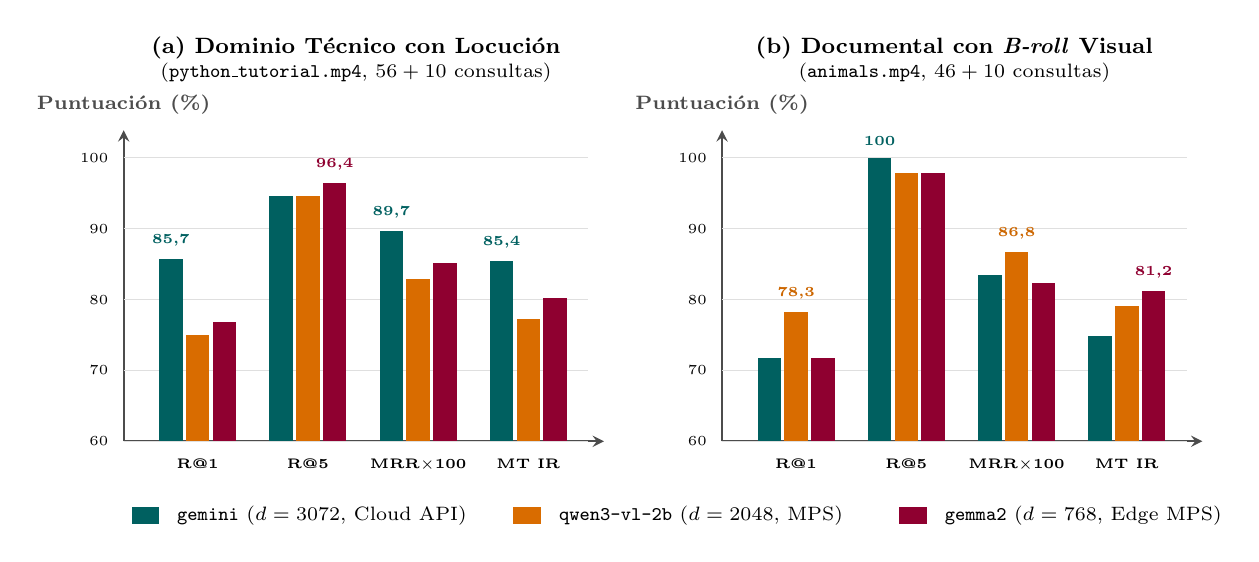
\begin{tikzpicture}
% Panel (a): python_tutorial.mp4
\begin{scope}
\draw[-stealth, thick, black!70] (0,0) -- (6.1,0);
\draw[-stealth, thick, black!70] (0,0) -- (0,3.95) node[above=2pt, font=\scriptsize\bfseries] {Puntuación (\%)};

% Líneas horizontales 60% a 100% (escala: (v - 60) * 0.09 cm)
\foreach \y/\lab in {0.0/60, 0.9/70, 1.8/80, 2.7/90, 3.6/100} {
    \draw[gray!25, thin] (0,\y) -- (5.9,\y);
    \node[left=2pt, font=\tiny] at (0,\y) {\lab};
}

% Grupo R@1 (x ~ 0.9), R@5 (x ~ 2.3), MRR (x ~ 3.7), MT IR (x ~ 5.1)
% Barras ancho 0.30, separacion 0.34
% Gemini (teal), Qwen (orange), Gemma (purple)
\fill[teal!75!black]    (0.45,0) rectangle (0.75,2.314);
\fill[orange!85!black]  (0.79,0) rectangle (1.09,1.350);
\fill[purple!75!black]  (1.13,0) rectangle (1.43,1.511);
\node[above=1pt, font=\tiny\bfseries, teal!75!black] at (0.60,2.314) {85,7};

\fill[teal!75!black]    (1.85,0) rectangle (2.15,3.118);
\fill[orange!85!black]  (2.19,0) rectangle (2.49,3.118);
\fill[purple!75!black]  (2.53,0) rectangle (2.83,3.279);
\node[above=1pt, font=\tiny\bfseries, purple!75!black] at (2.68,3.279) {96,4};

\fill[teal!75!black]    (3.25,0) rectangle (3.55,2.676);
\fill[orange!85!black]  (3.59,0) rectangle (3.89,2.060);
\fill[purple!75!black]  (3.93,0) rectangle (4.23,2.261);
\node[above=1pt, font=\tiny\bfseries, teal!75!black] at (3.40,2.676) {89,7};

\fill[teal!75!black]    (4.65,0) rectangle (4.95,2.288);
\fill[orange!85!black]  (4.99,0) rectangle (5.29,1.550);
\fill[purple!75!black]  (5.33,0) rectangle (5.63,1.825);
\node[above=1pt, font=\tiny\bfseries, teal!75!black] at (4.80,2.288) {85,4};

\node[below=3pt, font=\tiny\bfseries] at (0.94,0) {R@1};
\node[below=3pt, font=\tiny\bfseries] at (2.34,0) {R@5};
\node[below=3pt, font=\tiny\bfseries] at (3.74,0) {MRR$\times$100};
\node[below=3pt, font=\tiny\bfseries] at (5.14,0) {MT IR};

\node[font=\footnotesize\bfseries, align=center] at (2.95,4.85) {(a) Dominio Técnico con Locución\\[-1pt]{\scriptsize\normalfont(\texttt{python\_tutorial.mp4}, $56+10$ consultas)}};
\end{scope}

% Panel (b): animals.mp4
\begin{scope}[xshift=7.6cm]
\draw[-stealth, thick, black!70] (0,0) -- (6.1,0);
\draw[-stealth, thick, black!70] (0,0) -- (0,3.95) node[above=2pt, font=\scriptsize\bfseries] {Puntuación (\%)};

\foreach \y/\lab in {0.0/60, 0.9/70, 1.8/80, 2.7/90, 3.6/100} {
    \draw[gray!25, thin] (0,\y) -- (5.9,\y);
    \node[left=2pt, font=\tiny] at (0,\y) {\lab};
}

\fill[teal!75!black]    (0.45,0) rectangle (0.75,1.057);
\fill[orange!85!black]  (0.79,0) rectangle (1.09,1.643);
\fill[purple!75!black]  (1.13,0) rectangle (1.43,1.057);
\node[above=1pt, font=\tiny\bfseries, orange!80!black] at (0.94,1.643) {78,3};

\fill[teal!75!black]    (1.85,0) rectangle (2.15,3.600);
\fill[orange!85!black]  (2.19,0) rectangle (2.49,3.405);
\fill[purple!75!black]  (2.53,0) rectangle (2.83,3.405);
\node[above=1pt, font=\tiny\bfseries, teal!75!black] at (2.00,3.600) {100};

\fill[teal!75!black]    (3.25,0) rectangle (3.55,2.107);
\fill[orange!85!black]  (3.59,0) rectangle (3.89,2.410);
\fill[purple!75!black]  (3.93,0) rectangle (4.23,2.015);
\node[above=1pt, font=\tiny\bfseries, orange!80!black] at (3.74,2.410) {86,8};

\fill[teal!75!black]    (4.65,0) rectangle (4.95,1.340);
\fill[orange!85!black]  (4.99,0) rectangle (5.29,1.714);
\fill[purple!75!black]  (5.33,0) rectangle (5.63,1.911);
\node[above=1pt, font=\tiny\bfseries, purple!75!black] at (5.48,1.911) {81,2};

\node[below=3pt, font=\tiny\bfseries] at (0.94,0) {R@1};
\node[below=3pt, font=\tiny\bfseries] at (2.34,0) {R@5};
\node[below=3pt, font=\tiny\bfseries] at (3.74,0) {MRR$\times$100};
\node[below=3pt, font=\tiny\bfseries] at (5.14,0) {MT IR};

\node[font=\footnotesize\bfseries, align=center] at (2.95,4.85) {(b) Documental con \textit{B-roll} Visual\\[-1pt]{\scriptsize\normalfont(\texttt{animals.mp4}, $46+10$ consultas)}};
\end{scope}

% Leyenda compartida centrada abajo
\begin{scope}[yshift=-1.05cm, xshift=0.1cm]
\fill[teal!75!black]   (0.0,0) rectangle (0.35,0.22);
\node[right=3pt, font=\scriptsize] at (0.35,0.11) {\texttt{gemini} ($d=3072$, Cloud API)};
\fill[orange!85!black] (4.85,0) rectangle (5.20,0.22);
\node[right=3pt, font=\scriptsize] at (5.20,0.11) {\texttt{qwen3-vl-2b} ($d=2048$, MPS)};
\fill[purple!75!black] (9.75,0) rectangle (10.10,0.22);
\node[right=3pt, font=\scriptsize] at (10.10,0.11) {\texttt{gemma2} ($d=768$, Edge MPS)};
\end{scope}
\end{tikzpicture}
\caption{Comparativa de precisión inter-dominio en dimensión nativa (Etapa 1): \textit{Gemini Embedding 2} lidera el tutorial técnico basado en código y locución sincronizada, pero los modelos locales invierten la jerarquía en metraje documental con \textit{B-roll} visual desacoplado.}
\label{fig:backends_barras_interdominio}
\end{figure}

El análisis conjunto del Cuadro~\ref{tab:backends_metricas_por_dominio} y la Figura~\ref{fig:backends_barras_interdominio} evidencia una clara especialización arquitectónica entre dominios:

\begin{itemize}
    \item \textbf{Superioridad Cloud en discurso técnico estructurado (\texttt{python\_tutorial.mp4}):} \textit{Gemini} ($3072\text{d}$) logra el liderazgo indiscutible en \textit{Recall@1} ($85,71\%$, $+8,92\text{ pp}$ sobre \texttt{gemma2} y $+10,71\text{ pp}$ sobre \texttt{qwen3-vl-2b}) y \textit{MRR} ($0,8973$). Destaca que \texttt{gemma2} ($740\text{M}$ parámetros) supera sistemáticamente a \texttt{qwen3-vl-2b} ($2\text{B}$) en las cuatro métricas del tutorial técnico ($76,79\%$ vs. $75,00\%$ en \textit{Recall@1}; $92,86\%$ vs. $89,29\%$ en \textit{Recall@3}; $96,43\%$ vs. $94,64\%$ en \textit{Recall@5}; y $80,28\%$ vs. $77,22\%$ en \textit{Interval Recall}), lo que indica una alineación lingüística superior del tronco textual \textit{Gemma} frente a términos técnicos de programación en español integrados con la transcripción Whisper.

    \item \textbf{Inversión de rendimiento en metraje visual desacoplado (\texttt{animals.mp4}):} Cuando el audio narrativo describe categorías amplias mientras el fotograma muestra especies concretas, los codificadores visuales abiertos igualan o baten a la API remota. \textbf{\texttt{qwen3-vl-2b} obtiene los mejores registros absolutos del documental} en \textit{Recall@1} ($\mathbf{78,26\%}$, superando en $+6,52\text{ pp}$ a \textit{Gemini} y \textit{Gemma 2}), \textit{Recall@3} ($95,65\%$) y \textit{MRR} ($0,8678$), beneficiándose de su atención nativa sobre teselas visuales M-RoPE de $2\text{B}$ parámetros. Por su parte, \textbf{\texttt{gemma2} encabeza la recuperación multi-objetivo} (\texttt{top\_k=10}), elevando el \textit{Interval Recall} nativo al $\mathbf{81,23\%}$ (y hasta $\mathbf{85,15\%}$ en $512\text{d}/256\text{d}$), más de $10$ puntos porcentuales por encima de \texttt{gemini@3072} ($74,89\%$).

    \item \textbf{Competitividad global agregada ($102$ literales + $20$ multi-objetivo):} Agregando ambos vídeos, el modelo ligero \texttt{gemma2@768} iguala exactamente a \texttt{gemini@3072} tanto en \textit{Recall@3} ($\mathbf{93,14\%}$, $95/102$) como en \textit{Recall@5} ($\mathbf{97,06\%}$, $99/102$), y \texttt{gemma2@512} alcanza el mejor \textit{Interval Recall} multi-objetivo global de todo el estudio ($\mathbf{82,09\%}$ frente a $81,05\%$ de \texttt{gemini@768} y $80,31\%$ de \texttt{qwen3-vl-2b@1536}).
\end{itemize}

\paragraph{Significación Estadística Pareada Inter-Backend (\textit{McNemar} y \textit{Wilcoxon}):}
Los contrastes pareados sobre las puntuaciones por consulta confirman estadísticamente los resultados anteriores: en \texttt{python\_tutorial.mp4} ($N=56$), la ventaja de \texttt{gemini@3072} sobre \texttt{qwen3-vl-2b@2048} alcanza significación nominal en \textit{MRR} ($0,8973$ vs. $0,8289$, $p_{\text{Wilcoxon}} = 0,0396$; \textit{Recall@1} $p_{\text{McNemar}} = 0,1094$), mientras que ninguna otra pareja difiere significativamente ni en Python (\texttt{gemini@3072} vs. \texttt{gemma2@768}: $p_{\text{McNemar}} = 0,1797, p_{\text{Wilcoxon}} = 0,1605$; \texttt{qwen3-vl-2b@2048} vs. \texttt{gemma2@768}: $p_{\text{McNemar}} = 1,0000, p_{\text{Wilcoxon}} = 0,4864$) ni en \texttt{animals.mp4} ($N=46$, todos los contrastes con $p_{\text{McNemar}} \ge 0,5811$ y $p_{\text{Wilcoxon}} \ge 0,4721$). En el agregado global ($N=102$), los dos modelos locales logran \textbf{paridad estadística plena} frente al modelo comercial en la nube tanto en \texttt{qwen3-vl-2b@2048} vs. \texttt{gemini@3072} ($78/102$ vs. $81/102$, $p_{\text{McNemar}} = 0,6776, p_{\text{Wilcoxon}} = 0,2915$) como en \texttt{gemma2@768} vs. \texttt{gemini@3072} ($76/102$ vs. $81/102$, $p_{\text{McNemar}} = 0,3593, p_{\text{Wilcoxon}} = 0,2333$), y en igualdad dimensional entre \texttt{gemini@768} y \texttt{gemma2@768} ($80/102$ vs. $76/102$, $p_{\text{McNemar}} = 0,4807, p_{\text{Wilcoxon}} = 0,2796$).

\subsubsection{Curvas de Ablación Matryoshka (MRL) y Normalización \texorpdfstring{$L_2$}{L2}}
\label{subsubsec:curvas_mrl_normas}

Al evaluar la clase \texttt{Sentence\allowbreak Transformer} mediante el argumento \texttt{truncate\_\allowbreak dim} sobre Apple Silicon (\texttt{bfloat16}), se comprobó un detalle metodológico determinante: \textbf{dicho argumento recorta las primeras $d$ coordenadas sin renormalizar el vector resultante a la hiperesfera unitaria}. El Cuadro~\ref{tab:backends_normas_mrl} documenta las normas $L_2$ observadas tanto en una consulta aislada vía \texttt{truncate\_\allowbreak dim} como sobre los $164$ fragmentos reales de ambos vídeos antes de invocar \texttt{truncate\_\allowbreak and\_\allowbreak normalize\_\allowbreak mrl}.

\begin{table}[htbp]
\centering
\small
\setlength{\tabcolsep}{4.0pt}
\caption{Degradación empírica de la norma euclídea ($L_2$) en prefijos Matryoshka sin renormalizar frente a la restitución unitaria con \texttt{truncate\_and\_normalize\_mrl}.}
\label{tab:backends_normas_mrl}
\begin{adjustbox}{max width=\linewidth}
\begin{tabular}{lcccccc}
\toprule
\textbf{Backend} & \textbf{Dimensión ($d$)} & \textbf{Reducción} & \begin{tabular}[c]{@{}c@{}}\textbf{Norma \texttt{truncate\_dim}}\\\textbf{(consulta en MPS)}\end{tabular} & \begin{tabular}[c]{@{}c@{}}\textbf{Media $\|\mathbf{v}_{1:d}\|_2$}\\\textbf{(164 fragmentos)}\end{tabular} & \begin{tabular}[c]{@{}c@{}}\textbf{Rango $[\min,\max]$}\\\textbf{(164 fragmentos)}\end{tabular} & \begin{tabular}[c]{@{}c@{}}\textbf{Norma tras}\\\textbf{\texttt{truncate\_and\_normalize\_mrl}}\end{tabular} \\
\midrule
\texttt{gemini} & 3072 & $0,0\%$ & - & $1,0000$ & $[1,0000,\; 1,0000]$ & $\mathbf{1,0000}$ \\
\texttt{gemini} & 1536 & $50,0\%$ & - & $0,7267$ & $[0,7235,\; 0,7309]$ & $\mathbf{1,0000}$ \\
\texttt{gemini} & 768 & $75,0\%$ & - & $0,5612$ & $[0,5552,\; 0,5655]$ & $\mathbf{1,0000}$ \\
\midrule
\texttt{qwen3-vl-2b} & 2048 & $0,0\%$ & $1,0004$ & $1,0000$ & $[1,0000,\; 1,0000]$ & $\mathbf{1,0000}$ \\
\texttt{qwen3-vl-2b} & 1536 & $25,0\%$ & $0,8659$ & $0,8666$ & $[0,8450,\; 0,8858]$ & $\mathbf{1,0000}$ \\
\texttt{qwen3-vl-2b} & 768 & $62,5\%$ & $\mathbf{0,6284}$ & $\mathbf{0,6126}$ & $[0,5849,\; 0,6398]$ & $\mathbf{1,0000}$ \\
\midrule
\texttt{gemma2} & 768 & $0,0\%$ & $1,0016$ & $1,0000$ & $[1,0000,\; 1,0000]$ & $\mathbf{1,0000}$ \\
\texttt{gemma2} & 512 & $33,3\%$ & $0,8839$ & $0,8785$ & $[0,8684,\; 0,8854]$ & $\mathbf{1,0000}$ \\
\texttt{gemma2} & 256 & $66,7\%$ & $\mathbf{0,7152}$ & $\mathbf{0,7160}$ & $[0,7003,\; 0,7320]$ & $\mathbf{1,0000}$ \\
\bottomrule
\end{tabular}
\end{adjustbox}
\end{table}

Operar sin renormalizar reduce progresivamente la norma euclídea hasta valores medios de $0,7160$ en \texttt{gemma2@\allowbreak 256} ($0,7152$ en \texttt{truncate\_dim}) y $0,6126$ en \texttt{qwen3-vl-2b@\allowbreak 768} ($0,6284$ en \texttt{truncate\_dim}), distorsionando cualquier cálculo de producto escalar o umbralización fija y debilitando la estabilidad en cuantizaciones futuras (\texttt{int8}). Al delegar el corte en \texttt{truncate\_and\_\allowbreak normalize\_mrl}, todos los vectores recuperan estrictamente $\|\hat{\mathbf{v}}\|_2 = 1,0$.

La Figura~\ref{fig:backends_curvas_mrl} traza las curvas globales de retención Matryoshka sobre las $102$ consultas literales y las $20$ multi-objetivo en función del ahorro efectivo de memoria en Qdrant.

\begin{figure}[htbp]
\centering
\begin{tikzpicture}
% Panel (a): Recall@1 Global (102 consultas) vs Ahorro MRL (%)
\begin{scope}
\draw[-stealth, thick, black!70] (0,0) -- (5.5,0);
\draw[-stealth, thick, black!70] (0,0) -- (0,3.8) node[above=2pt, font=\scriptsize\bfseries] {Recall@1 Global (\%)};

% Eje Y: 70% a 82% -> (v - 70) * 0.28 cm
\foreach \y/\lab in {0.0/70\%, 0.84/73\%, 1.68/76\%, 2.52/79\%, 3.36/82\%} {
    \draw[gray!25, thin] (0,\y) -- (5.2,\y);
    \node[left=2pt, font=\tiny] at (0,\y) {\lab};
}
% Eje X: Ahorro 0% a 80% -> sav * 0.065 cm
\foreach \x/\lab in {0.0/0\%, 1.625/25\%, 3.25/50\%, 4.875/75\%} {
    \draw[gray!30, thin] (\x,0) -- (\x,3.36);
    \node[below=2pt, font=\tiny] at (\x,0) {\lab};
}
\node[below=14pt, font=\scriptsize\bfseries] at (2.6,0) {Ahorro de Almacenamiento (\%)};

% Curva Gemini: (0, 2.635), (3.250, 2.360), (4.875, 2.360)
\draw[very thick, teal!75!black] (0.000,2.635) -- (3.250,2.360) -- (4.875,2.360);
\foreach \x/\y in {0.000/2.635, 3.250/2.360, 4.875/2.360} {
    \fill[teal!75!black] (\x,\y) circle (2.2pt);
}
\node[above right=1pt and 2pt, font=\tiny\bfseries, teal!75!black] at (0.0,2.635) {79,4\% (3072d)};
\node[above=3pt, font=\tiny\bfseries, teal!75!black] at (4.65,2.360) {78,4\% (768d)};

% Curva Qwen3-VL-2B: (0, 1.812), (1.625, 1.812), (4.062, 1.812)
\draw[very thick, orange!85!black] (0.000,1.812) -- (1.625,1.812) -- (4.062,1.812);
\foreach \x/\y in {0.000/1.812, 1.625/1.812, 4.062/1.812} {
    \node[fill=orange!85!black, minimum size=4pt, inner sep=0pt] at (\x,\y) {};
}
\node[above right=2pt and 2pt, font=\tiny\bfseries, orange!80!black] at (0.0,1.812) {76,5\% (2048d $\to$ 768d invariante)};

% Curva Gemma 2: (0, 1.263), (2.164, 1.263), (4.336, 0.988)
\draw[very thick, purple!75!black] (0.000,1.263) -- (2.164,1.263) -- (4.336,0.988);
\foreach \x/\y in {0.000/1.263, 2.164/1.263, 4.336/0.988} {
    \node[regular polygon, regular polygon sides=3, fill=purple!75!black, minimum size=4.6pt, inner sep=0pt] at (\x,\y) {};
}
\node[below right=1pt and 2pt, font=\tiny\bfseries, purple!75!black] at (0.0,1.263) {74,5\% (768d / 512d)};
\node[below=3pt, font=\tiny\bfseries, purple!75!black] at (4.336,0.988) {73,5\% (256d)};

\node[font=\footnotesize\bfseries, align=center] at (2.6,4.75) {(a) Retención \textit{Recall@1} Literal\\[-1pt]{\scriptsize\normalfont(102 consultas agregadas)}};
\end{scope}

% Panel (b): MT Interval Recall Etapa 1 (20 consultas) vs Ahorro MRL (%)
\begin{scope}[xshift=7.7cm]
\draw[-stealth, thick, black!70] (0,0) -- (5.5,0);
\draw[-stealth, thick, black!70] (0,0) -- (0,3.8) node[above=2pt, font=\scriptsize\bfseries] {MT Interval Recall (\%)};

% Eje Y: 75% a 85% -> (v - 75) * 0.336 cm
\foreach \y/\lab in {0.0/75\%, 0.84/77{,}5\%, 1.68/80\%, 2.52/82{,}5\%, 3.36/85\%} {
    \draw[gray!25, thin] (0,\y) -- (5.2,\y);
    \node[left=2pt, font=\tiny] at (0,\y) {\lab};
}
\foreach \x/\lab in {0.0/0\%, 1.625/25\%, 3.25/50\%, 4.875/75\%} {
    \draw[gray!30, thin] (\x,0) -- (\x,3.36);
    \node[below=2pt, font=\tiny] at (\x,0) {\lab};
}
\node[below=14pt, font=\scriptsize\bfseries] at (2.6,0) {Ahorro de Almacenamiento (\%)};

% Curva Gemini: (0, 1.730), (3.250, 1.522), (4.875, 2.033)
\draw[very thick, teal!75!black] (0.000,1.730) -- (3.250,1.522) -- (4.875,2.033);
\foreach \x/\y in {0.000/1.730, 3.250/1.522, 4.875/2.033} {
    \fill[teal!75!black] (\x,\y) circle (2.2pt);
}
\node[above=3pt, font=\tiny\bfseries, teal!75!black] at (4.70,2.033) {81,1\%};

% Curva Qwen3-VL-2B: (0, 1.052), (1.625, 1.784), (4.062, 0.706)
\draw[very thick, orange!85!black] (0.000,1.052) -- (1.625,1.784) -- (4.062,0.706);
\foreach \x/\y in {0.000/1.052, 1.625/1.784, 4.062/0.706} {
    \node[fill=orange!85!black, minimum size=4pt, inner sep=0pt] at (\x,\y) {};
}
\node[below=3pt, font=\tiny\bfseries, orange!80!black] at (4.062,0.706) {77,1\%};
\node[font=\tiny\bfseries, orange!80!black] (qmid) at (2.00,1.12) {80,3\% (1536d)};
\draw[orange!75!black, very thin] (1.625,1.784) -- (qmid.north);

% Curva Gemma 2: (0, 1.932), (2.164, 2.382), (4.336, 1.683)
\draw[very thick, purple!75!black] (0.000,1.932) -- (2.164,2.382) -- (4.336,1.683);
\foreach \x/\y in {0.000/1.932, 2.164/2.382, 4.336/1.683} {
    \node[regular polygon, regular polygon sides=3, fill=purple!75!black, minimum size=4.6pt, inner sep=0pt] at (\x,\y) {};
}
\node[above=3pt, font=\tiny\bfseries, purple!75!black] at (2.164,2.382) {82,1\% (512d)};
\node[above right=2pt and 1pt, font=\tiny\bfseries, purple!75!black] at (0.0,1.932) {80,8\%};

\node[font=\footnotesize\bfseries, align=center] at (2.6,4.75) {(b) \textit{Interval Recall} Multi-Objetivo\\[-1pt]{\scriptsize\normalfont(20 consultas, Etapa 1 \texttt{top\_k=10})}};
\end{scope}

% Leyenda compartida
\begin{scope}[yshift=-1.28cm, xshift=2.2cm]
\draw[very thick, teal!75!black] (0.0,0.1) -- (0.5,0.1);
\fill[teal!75!black] (0.25,0.1) circle (2.2pt);
\node[right=3pt, font=\scriptsize] at (0.5,0.1) {\texttt{gemini}};

\draw[very thick, orange!85!black] (3.4,0.1) -- (3.9,0.1);
\node[fill=orange!85!black, minimum size=4pt, inner sep=0pt] at (3.65,0.1) {};
\node[right=3pt, font=\scriptsize] at (3.9,0.1) {\texttt{qwen3-vl-2b}};

\draw[very thick, purple!75!black] (7.2,0.1) -- (7.7,0.1);
\node[regular polygon, regular polygon sides=3, fill=purple!75!black, minimum size=4.6pt, inner sep=0pt] at (7.45,0.1) {};
\node[right=3pt, font=\scriptsize] at (7.7,0.1) {\texttt{gemma2}};
\end{scope}
\end{tikzpicture}
\caption{Curvas de ablación Matryoshka (MRL) globales: \texttt{qwen3-vl-2b} exhibe invarianza perfecta del $100\%$ en \textit{Recall@1} ($76,5\%$) desde $2048\text{d}$ hasta $768\text{d}$, mientras que \texttt{gemma2@512} alcanza el máximo global de \textit{Interval Recall} multi-objetivo ($82,1\%$) y conserva $73,5\%$ de \textit{Recall@1} incluso a $256\text{d}$ ($1\text{ KB/chunk}$).}
\label{fig:backends_curvas_mrl}
\end{figure}

El análisis de las trayectorias Matryoshka arroja tres resultados notables:
\begin{enumerate}
    \item \textbf{Invarianza en \texttt{qwen3-vl-2b}:} Mantiene exactamente $76,47\%$ ($78/102$) de \textit{Recall@1} y $92,16\%$ ($94/102$) de \textit{Recall@3} en $2048\text{d}$, $1536\text{d}$ y $768\text{d}$ ($-62,5\%$ de espacio), además de mejorar el \textit{Interval Recall} multi-objetivo en $1536\text{d}$ ($80,31\%$ frente a $78,13\%$ en $2048\text{d}$).
    \item \textbf{Eficiencia extrema en \texttt{gemma2@256}:} Con un tamaño de almacenamiento de tan solo $1,00\text{ KB/chunk}$ ($82,00\text{ KB}$ por vídeo frente a $984,00\text{ KB}$ en \texttt{gemini@3072}, una reducción de $12\times$), \texttt{gemma2@256} solo cede un acierto en \textit{Recall@1} respecto a $768\text{d}$ ($75/102$ frente a $76/102$) y conserva $80,01\%$ de \textit{Interval Recall} multi-objetivo.
    \item \textbf{Efecto regularizador en sub-dimensiones intermedias:} Igual que \texttt{gemini} maximiza \textit{Recall@5} ($99,02\%$) y \textit{MT IR} ($81,05\%$) en $768\text{d}$, tanto \texttt{qwen3-vl-2b@1536} como \texttt{gemma2@512} logran sus picos multi-objetivo ($80,31\%$ y $82,09\%$) en dimensión reducida, confirmando que descartar las dimensiones finales de baja varianza mitiga sobreajustes locales en búsquedas de múltiple objetivo.
\end{enumerate}

Desde el punto de vista inferencial ($N=102$), la compresión desde la dimensión nativa hasta la mínima evaluada en cada motor no produce pérdida estadísticamente significativa ni en \textit{Recall@1} ni en \textit{MRR}: \texttt{gemini} ($3072\text{d} \to 768\text{d}$: $p_{\text{McNemar}} = 1,0000, p_{\text{Wilcoxon}} = 0,6729$), \texttt{qwen3-vl-2b} ($2048\text{d} \to 768\text{d}$: $p_{\text{McNemar}} = 1,0000, p_{\text{Wilcoxon}} = 0,5519$) y \texttt{gemma2} ($768\text{d} \to 256\text{d}$: $p_{\text{McNemar}} = 1,0000, p_{\text{Wilcoxon}} = 0,4370$).

\subsubsection{Rendimiento Computacional, Latencia y Huella de Memoria}
\label{subsubsec:rendimiento_memoria_backends}

El Cuadro~\ref{tab:backends_coste_recursos} consolida los costes de indexación, tiempos de respuesta en consulta y consumo máximo de memoria RAM (\texttt{RSS}) y gráfica integrada (\texttt{MPS driver\_allocated\_memory}), complementado visualmente por la Figura~\ref{fig:backends_tradeoff_latencia_memoria}.

\begin{table}[htbp]
\centering
\small
\setlength{\tabcolsep}{3.5pt}
\caption{Rendimiento computacional, latencia de consulta y huella máxima de memoria por vídeo y backend (configuraciones nativas).}
\label{tab:backends_coste_recursos}
\begin{adjustbox}{max width=\linewidth}
\begin{tabular}{llccccccc}
\toprule
\textbf{Corpus} & \textbf{Backend (Dim)} & \textbf{Dispositivo} & \begin{tabular}[c]{@{}c@{}}\textbf{Indexación}\\\textbf{Total}\end{tabular} & \begin{tabular}[c]{@{}c@{}}\textbf{Coste /}\\\textbf{Fragmento}\end{tabular} & \begin{tabular}[c]{@{}c@{}}\textbf{Consulta}\\\textbf{Media (ms)}\end{tabular} & \begin{tabular}[c]{@{}c@{}}\textbf{Consulta}\\\textbf{Mediana (ms)}\end{tabular} & \begin{tabular}[c]{@{}c@{}}\textbf{Pico RSS}\\\textbf{(MB)}\end{tabular} & \begin{tabular}[c]{@{}c@{}}\textbf{Pico MPS}\\\textbf{(MB)}\end{tabular} \\
\midrule
\multirow{3}{*}{\texttt{python\_tutorial.mp4}}
 & \texttt{gemini} ($3072$) & Cloud API & $227,31\text{ s}$ & $2,772\text{ s}$ & $484,67$ & $481,30$ & $391,4$ & $0$ \\
 & \texttt{qwen3-vl-2b} ($2048$) & Local MPS & $\mathbf{142,23\text{ s}}$ & $\mathbf{1,734\text{ s}}$ & $95,11$ & $97,69$ & $2.095,1$ & $4.736,5$ \\
 & \texttt{gemma2} ($768$) & Local MPS & $247,73\text{ s}$ & $3,021\text{ s}$ & $\mathbf{30,11}$ & $\mathbf{29,93}$ & $3.081,5$ & $\mathbf{2.552,6}$ \\
\midrule
\multirow{3}{*}{\texttt{animals.mp4}}
 & \texttt{gemini} ($3072$) & Cloud API & $187,12\text{ s}$ & $2,282\text{ s}$ & $1.086,72^*$ & $464,18$ & $424,0$ & $0$ \\
 & \texttt{qwen3-vl-2b} ($2048$) & Local MPS & $\mathbf{126,05\text{ s}}$ & $\mathbf{1,537\text{ s}}$ & $92,33$ & $90,94$ & $1.995,8$ & $4.737,7$ \\
 & \texttt{gemma2} ($768$) & Local MPS & $245,49\text{ s}$ & $2,994\text{ s}$ & $\mathbf{31,08}$ & $\mathbf{30,20}$ & $2.641,2$ & $\mathbf{2.592,1}$ \\
\bottomrule
\end{tabular}
\end{adjustbox}
\vspace{2pt}
{\scriptsize $^*$Incluye picos puntuales de latencia TLS/API remota; la mediana ($464,18\text{ ms}$) representa el tiempo típico de respuesta en red.}
\end{table}

\begin{figure}[htbp]
\centering
\begin{tikzpicture}
% Panel (a): Latencia consulta mediana (ms) vs Coste indexacion (s/chunk)
\begin{scope}
\draw[-stealth, thick, black!70] (0,0) -- (5.5,0);
\draw[-stealth, thick, black!70] (0,0) -- (0,3.8) node[above=2pt, font=\scriptsize\bfseries] {Indexación (s/chunk)};

% Y: 0 a 3.5 s/chunk (escala 1.0 cm por s/chunk)
\foreach \y/\lab in {1.0/1{,}0, 2.0/2{,}0, 3.0/3{,}0} {
    \draw[gray!25, thin] (0,\y) -- (5.3,\y);
    \node[left=2pt, font=\tiny] at (0,\y) {\lab};
}
% X: 0 a 550 ms (escala 0.01 cm/ms)
\foreach \x/\lab in {1.0/100, 2.5/250, 4.0/400, 5.0/500} {
    \draw[gray!25, thin] (\x,0) -- (\x,3.5);
    \node[below=2pt, font=\tiny] at (\x,0) {\lab};
}
\node[below=14pt, font=\scriptsize\bfseries] at (2.7,0) {Mediana Consulta (ms)};

% Zona optima Pareto esquina inferior izquierda
\fill[green!12, rounded corners=3pt] (0.05,0.05) rectangle (1.45,1.95);
\node[font=\tiny\itshape, green!50!black] at (0.75,0.30) {Frente local rápido};

% Gemma2: Py (0.299, 3.021), An (0.302, 2.994)
\node[regular polygon, regular polygon sides=3, fill=purple!75!black, minimum size=5pt, inner sep=0pt] (gpy) at (0.299,3.021) {};
\node[regular polygon, regular polygon sides=3, draw=purple!75!black, fill=white, thick, minimum size=5pt, inner sep=0pt] (gan) at (0.302,2.994) {};
\node[right=4pt, font=\tiny\bfseries, purple!75!black, align=left] at (0.35,3.05) {\texttt{gemma2}\\($\sim 30\text{ ms}$, $3,0\text{ s/c}$)};

% Qwen: Py (0.977, 1.734), An (0.909, 1.537)
\node[fill=orange!85!black, minimum size=4.5pt, inner sep=0pt] (qpy) at (0.977,1.734) {};
\node[draw=orange!85!black, fill=white, thick, minimum size=4.5pt, inner sep=0pt] (qan) at (0.909,1.537) {};
\node[right=4pt, font=\tiny\bfseries, orange!80!black, align=left] at (1.05,1.65) {\texttt{qwen3-vl-2b}\\($91$--$98\text{ ms}$, $1,5$--$1,7\text{ s/c}$)};

% Gemini: Py (4.813, 2.772), An (4.642, 2.282)
\fill[teal!75!black] (4.813,2.772) circle (2.4pt);
\draw[teal!75!black, fill=white, thick] (4.642,2.282) circle (2.4pt);
\node[left=4pt, font=\tiny\bfseries, teal!75!black, align=right] at (4.60,2.55) {\texttt{gemini} Cloud\\($464$--$481\text{ ms}$, $2,3$--$2,8\text{ s/c}$)};

\node[font=\footnotesize\bfseries, align=center] at (2.7,4.75) {(a) Latencia de Consulta vs. Indexación\\[-1pt]{\scriptsize\normalfont(Símbolo sólido: Python; hueco: Animals)}};
\end{scope}

% Panel (b): Pico de Memoria RSS vs GPU Metal (MPS)
\begin{scope}[xshift=7.8cm]
\draw[-stealth, thick, black!70] (0,0) -- (5.3,0);
\draw[-stealth, thick, black!70] (0,0) -- (0,3.8) node[above=2pt, font=\scriptsize\bfseries] {Memoria Pico (MB)};

% Escala Y: 1 cm = 1500 MB (hasta 5000 MB -> 3.33 cm)
\foreach \y/\lab in {1.0/1.500, 2.0/3.000, 3.0/4.500} {
    \draw[gray!25, thin] (0,\y) -- (5.1,\y);
    \node[left=2pt, font=\tiny] at (0,\y) {\lab};
}

% Grupo Gemini (x=0.8), Qwen (x=2.4), Gemma (x=4.0), media Py/An:
% Gemini: RSS=408 (0.272), MPS=0
\fill[blue!70!black] (0.50,0) rectangle (0.90,0.272);
\fill[magenta!75!black] (0.94,0) rectangle (1.34,0.020);
\node[above=1pt, font=\tiny\bfseries, blue!70!black] at (0.68,0.272) {408};
\node[above=1pt, font=\tiny, magenta!75!black] at (1.14,0.03) {0};

% Qwen: RSS=2045 (1.363), MPS=4737 (3.158)
\fill[blue!70!black] (2.10,0) rectangle (2.50,1.363);
\fill[magenta!75!black] (2.54,0) rectangle (2.94,3.158);
\node[above=1pt, font=\tiny\bfseries, blue!70!black] at (2.22,1.363) {2.045};
\node[above=1pt, font=\tiny\bfseries, magenta!75!black] at (2.74,3.158) {4.737};

% Gemma2: RSS=2861 (1.908), MPS=2572 (1.715)
\fill[blue!70!black] (3.70,0) rectangle (4.10,1.908);
\fill[magenta!75!black] (4.14,0) rectangle (4.54,1.715);
\node[above=1pt, font=\tiny\bfseries, blue!70!black] at (3.82,1.908) {2.861};
\node[above=1pt, font=\tiny\bfseries, magenta!75!black] at (4.42,1.715) {2.572};

\node[below=3pt, font=\scriptsize\bfseries] at (0.92,0) {\texttt{gemini}};
\node[below=3pt, font=\scriptsize\bfseries] at (2.52,0) {\texttt{qwen3-vl-2b}};
\node[below=3pt, font=\scriptsize\bfseries] at (4.12,0) {\texttt{gemma2}};

% Leyenda b
\fill[blue!70!black]    (-0.10,-0.85) rectangle (0.20,-0.65);
\node[right=2pt, font=\tiny] at (0.20,-0.75) {RSS Proceso (promedio)};
\fill[magenta!75!black] (3.00,-0.85) rectangle (3.30,-0.65);
\node[right=2pt, font=\tiny] at (3.30,-0.75) {GPU Driver Metal (MPS)};

\node[font=\footnotesize\bfseries, align=center] at (2.55,4.75) {(b) Huella Física de Memoria\\[-1pt]{\scriptsize\normalfont(Media entre ambos corpus en $16\text{ GB}$)}};
\end{scope}
\end{tikzpicture}
\caption{Compromiso entre rendimiento temporal y recursos de memoria en Apple Silicon M3 ($16\text{ GB}$): \texttt{gemma2} reduce la latencia de consulta local en un factor de $15$--$16\times$ frente a Cloud API consumiendo casi la mitad de memoria MPS que \texttt{qwen3-vl-2b}, mientras que \texttt{qwen3-vl-2b} consigue la indexación de vídeo más veloz.}
\label{fig:backends_tradeoff_latencia_memoria}
\end{figure}

La comparativa temporal y de recursos revela tres hallazgos clave de ingeniería:
\begin{enumerate}
    \item \textbf{Aceleración interactiva de hasta $16\times$ en consultas locales:} Al eliminar el viaje de red HTTP/TLS hasta los servidores de la API Cloud (mediana de $464,18$--$481,30\text{ ms}$), \texttt{qwen3-vl-2b} responde en $90,94$--$97,69\text{ ms}$ ($\approx 5\times$ más rápido) y \texttt{gemma2} en apenas $\mathbf{29,93}$--$\mathbf{30,20\text{ ms}}$ ($15,4\times$--$16,1\times$ más rápido). Esto permite ejecutar búsquedas vectoriales en Qdrant en tiempo casi instantáneo de percepción humana ($< 35\text{ ms}$ totales).
    \item \textbf{Asimetría arquitectónica entre consulta textual e indexación de fotogramas:} Aunque \texttt{gemma2} es $3\times$ más rápido en consultas de texto ($23,6\text{ ms}$ frente a $72,9\text{ ms}$ medidos en aislamiento sobre MPS tras \texttt{torch.mps.synchronize()}), porque en texto puro activa únicamente su tronco lingüístico de $270\text{M}$ parámetros, al indexar fragmentos multimodales de $3$ fotogramas ($512\text{ px}$) invoca su codificador visual ($170\text{M}$) con un coste neto de $1.960,1\text{ ms/chunk}$ frente a $1.180,6\text{ ms/chunk}$ en \texttt{qwen3-vl-2b}. Sumando las etapas constantes de segmentación SSIM y transcripción Whisper, \textbf{\texttt{qwen3-vl-2b} completa la indexación de un vídeo en $126,05$--$142,23\text{ s}$}, superando incluso a \textit{Gemini Cloud} ($187,12$--$227,31\text{ s}$).
    \item \textbf{Contención en $16\text{ GB}$ unificados:} Al combinar la descarga de Whisper con \texttt{Semaphore(1)}, ningún motor local bloquea el equipo: \texttt{gemma2} opera con apenas $\mathbf{2,55\text{--}2,59\text{ GB}}$ \textbf{de memoria GPU Metal} ($46\%$ menos que \texttt{qwen3-vl-2b}, con $4,74\text{ GB}$), posicionándose como la alternativa óptima para portátiles o despliegue en el borde con restricciones estrictas de VRAM compartida.
\end{enumerate}

\subsubsection{Criterios de Selección Arquitectónica Cloud vs. Local}
A la luz de la evidencia recopilada en ambos vídeos, no existe un ganador absoluto en todas las dimensiones operativas, sino un espectro complementario claro:
\begin{itemize}
    \item \textbf{Escenarios sin GPU o de discurso técnico denso:} \texttt{gemini@768} mantiene el mejor equilibrio global de precisión en Etapa 1 en contenido hablado/código ($85,71\%$ \textit{Recall@1} en Python) con huella local prácticamente nula ($391-424\text{ MB}$ RSS), a costa de $464-481\text{ ms}$ de red y sujeción a cuotas RPD.
    \item \textbf{Búsqueda visual en metraje documental o alta velocidad de ingesta privada:} \texttt{qwen3-vl-2b@\allowbreak 1536} ofrece la mejor combinación de precisión puramente visual ($78,26\%$ \textit{Recall@1} y $81,31\%$ \textit{MT IR} en \texttt{animals.mp4}) y el menor tiempo de indexación ($1,54-1,73\text{ s/chunk}$) sin cuotas externas, asumiendo $\approx 4,74\text{ GB}$ de memoria Metal.
    \item \textbf{Computación Edge, baja latencia y mínimo almacenamiento:} Las variantes \texttt{gemma2@\allowbreak 512} y \texttt{gemma2@\allowbreak 256} ejecutan consultas locales en $\approx 30\text{ ms}$ consumiendo solo $2,55-2,59\text{ GB}$ de MPS, lideran el \textit{Interval Recall} multi-objetivo global ($82,09\%$ en $512\text{d}$) y reducen la base vectorial hasta $1,00\text{ KB/chunk}$ ($82\text{ KB}$ por vídeo).
\end{itemize}

